% MRIxFields 2026: Progress Report III. Everything between Progress Report II (end of August
% 2026) and the final ranking (October 2026), self-contained: the figures and tables of the
% architecture log, the decision tree and the error-spectrum log are reproduced here.
% Numbers: validation phase = challenge leaderboard; test phase = Synapse "Final Ranking"
% (syn72060672, 1 Oct 2026); local = three paired subjects, fixed harness only. Section numbers
% in brackets are TODO.md.
% Compile from inside reports/:  ~/anaconda3/envs/tex/bin/tectonic changes_since_slides2.tex
\documentclass[10pt,a4paper]{article}

\usepackage[margin=18mm]{geometry}
\usepackage[T1]{fontenc}
\usepackage{booktabs}
\usepackage{xcolor}
\usepackage{graphicx}
\usepackage{caption}
\usepackage{subcaption}
\usepackage{float}
\usepackage{amsmath}
\usepackage{amssymb}
\usepackage{enumitem}
\usepackage{tikz}
\usepackage[colorlinks=true,linkcolor=black,urlcolor=black]{hyperref}
\usetikzlibrary{positioning,arrows.meta,fit,backgrounds,calc}

\definecolor{base}{HTML}{9FB3C8}
\definecolor{baseline}{HTML}{D9E2EC}
\definecolor{accent}{HTML}{D64545}
\definecolor{accentfill}{HTML}{FBE4E4}
\definecolor{cond}{HTML}{3E7CB1}
\definecolor{ink}{HTML}{102A43}
\definecolor{muted}{HTML}{627D98}
\definecolor{keep}{HTML}{2C7A5A}
\definecolor{keepfill}{HTML}{E8F3ED}
\definecolor{drop}{HTML}{9AA5B1}
\definecolor{dropfill}{HTML}{F5F7FA}
\definecolor{live}{HTML}{B45309}
\definecolor{livefill}{HTML}{FDF3E3}

\captionsetup[figure]{font=small,labelfont=bf}
\captionsetup[table]{font=small,labelfont=bf}
\captionsetup[subfigure]{font=small}
\setlist[itemize]{itemsep=0.6mm,topsep=1mm}
\setlength{\parindent}{0pt}
\setlength{\parskip}{1.2mm}

\newcommand{\da}{\Delta\alpha}
\newcommand{\pending}[1][pending]{\textcolor{live}{\textit{#1}}}
\newcommand{\statkept}{\textcolor{keep}{\textbf{kept}}}
\newcommand{\statdropped}{\textcolor{accent}{\textbf{dropped}}}
\newcommand{\statopen}{\textcolor{live}{\textbf{open}}}

% ---------------------------------------------------------------- U-Net glyph (architecture log)
\tikzset{
  blk/.style   = {draw=base, fill=baseline, rounded corners=0.4pt,
                  minimum height=2.4mm, inner sep=0pt, line width=0.3pt},
  hot/.style   = {draw=accent, fill=accentfill, line width=0.7pt},
  io/.style    = {font=\tiny, text=muted, inner sep=1pt},
  skip/.style  = {->, draw=base, line width=0.3pt, >={Stealth[length=1mm]}},
  flow/.style  = {->, draw=muted, line width=0.35pt, >={Stealth[length=1.2mm]}},
  tag/.style   = {font=\tiny\bfseries, text=accent, inner sep=1pt},
}

\newcommand{\unet}[1]{%
\begin{tikzpicture}[x=1mm,y=1mm,baseline]
  % fixed bounding box: every glyph is the same size, so the captions below line up
  \path (-9.5,9.5) rectangle (24,-23);
  % encoder (left) and decoder (right); each level is indented, so the shape reads as a U
  \foreach \i/\w in {0/9,1/7,2/5,3/3.5}{
    \node[blk,minimum width=\w mm] (e\i) at ({\i*1.7},{-\i*4}) {};
    \node[blk,minimum width=\w mm] (d\i) at ({16-\i*1.7},{-\i*4}) {};
  }
  \node[blk,minimum width=3mm] (b) at (8,-16.5) {};
  \foreach \i in {0,1,2,3}{ \draw[skip] (e\i) -- (d\i); }
  \foreach \i [evaluate=\i as \j using int(\i+1)] in {0,1,2}{
    \draw[flow] (e\i) -- (e\j);  \draw[flow] (d\j) -- (d\i);
  }
  \draw[flow] (e3) -- (b);  \draw[flow] (b) -- (d3);
  \node[io,left=1.2mm of e0] (in) {$x$};
  \node[io,right=1.2mm of d0] (out) {$\hat{y}$};
  \draw[flow] (in) -- (e0);  \draw[flow] (d0) -- (out);
  #1
\end{tikzpicture}}

% conditioning tokens added at the bottleneck
\newcommand{\condtokens}[1][cond]{%
  \node[draw=#1, fill=white, rounded corners=0.4pt, minimum width=7mm,
        minimum height=2.2mm, line width=0.5pt, font=\tiny, text=#1,
        inner sep=0.5pt] (c) at (8,-21) {$E_s\!+\!E_t$};
  \draw[->, draw=#1, line width=0.5pt, >={Stealth[length=1mm]}] (c) -- (b);}

% panel heading: short name left, score right, always one line
\newcommand{\panel}[2]{\makebox[\linewidth]{\footnotesize\bfseries #1\hfill #2}}

% ---------------------------------------------------------------- decision tree (renamed macros)
\tikzset{
  kept/.style = {draw=keep, fill=keepfill, line width=0.7pt, rounded corners=1.2pt,
                 text width=44mm, inner sep=1.6mm, align=left, font=\footnotesize},
  gone/.style = {draw=drop, fill=dropfill, line width=0.4pt, dashed, rounded corners=1.2pt,
                 text width=58mm, inner sep=1.3mm, align=left, font=\scriptsize, text=muted},
  back/.style = {draw=keep, fill=dropfill, line width=0.5pt, dashed, rounded corners=1.2pt,
                 text width=58mm, inner sep=1.3mm, align=left, font=\scriptsize, text=keep},
  now/.style  = {draw=live, fill=livefill, line width=0.7pt, rounded corners=1.2pt,
                 text width=44mm, inner sep=1.5mm, align=left, font=\footnotesize},
  spine/.style = {->, draw=keep, line width=1.1pt, >={Stealth[length=2mm]}},
  stub/.style  = {->, draw=drop, line width=0.4pt, dashed, >={Stealth[length=1.4mm]}},
  ret/.style   = {->, draw=keep, line width=0.5pt, dashed, >={Stealth[length=1.4mm]}},
  sec/.style   = {font=\footnotesize\bfseries, text=ink},
}

% #1 node name, #2 y, #3 section, #4 what it was, #5 result
\newcommand{\dtkept}[5]{\node[kept] (#1) at (0,#2)
  {{\bfseries #3}~~#4\\[0.4mm]{\bfseries\color{keep}#5}};}
\newcommand{\dtgone}[5]{\node[gone] (#1) at (7.6,#2)
  {\hyphenpenalty=10000\exhyphenpenalty=10000\relax
   {\bfseries #3}~~#4 \hfill \textbf{#5}};}
\newcommand{\dtback}[5]{\node[back] (#1) at (7.6,#2)
  {\hyphenpenalty=10000\exhyphenpenalty=10000\relax
   {\bfseries #3}~~#4 \hfill \textbf{#5}};}
\newcommand{\dtnote}[2]{\node[font=\scriptsize\itshape, text=muted, text width=34mm, align=right]
  at (-4.4,#1) {#2};}

\title{\bfseries MRIxFields 2026: Progress Report III\\[0.3em]
\large Task 3, from Report II to the final ranking}
\author{Berkin Deniz Kahya \and Furkan Y\"uceyal\c{c}\i n \and Racha Badreddine \and Ahmet Zelka}
\date{8 October 2026}

\begin{document}
\sloppy
\maketitle

% ======================================================================
\section{Summary}\label{sec:summary}

\begin{itemize}
  \item \textbf{Result.} 3rd Place Award, Task 3 (top 9 of 25 teams). Final test phase (20 unseen
        volunteers, Docker submission): SSIM \textbf{0.942551, 4th} on the challenge's main
        metric; nRMSE 0.248030, 6th; LPIPS 0.050566, 14th; mean rank 8.00, 6th (tied). Presented
        at the MRIxFields 2026 workshop, MICCAI 2026, Strasbourg, 1 October 2026
        (Section~\ref{sec:final}).
  \item \textbf{Validation line.} Report II's best Task 3 model, the 10-epoch conditional U-Net,
        scored SSIM 0.9014. The shipped model scores \textbf{0.913652}: a 32-channel conditional
        U-Net, MIM-pretrained on 1{,}939 unpaired volumes, given all three contrasts, trained with
        SSIM in the loss, with an axial-position token, three checkpoints averaged and four flips
        (Section~\ref{sec:model}).
  \item \textbf{What moved it} was information the network sees, then averaging: which domain pair
        $+0.0278$, unpaired data $+0.0103$, the other two contrasts $+0.0037$, the metric in the
        loss $+0.0021$, averaging and flips $+0.0042$. Five other backbones and formulations
        scored 0.858 to 0.887 (Sections~\ref{sec:model} and~\ref{sec:other}).
  \item \textbf{Measurement.} Until 2026-09-11 the local harness scored sagittal planes; every
        local number before that date is void (Section~\ref{sec:measure}). Two decisions it
        caused were reversed on the leaderboard.
  \item \textbf{Where the error is.} 0.1\,T is 40\% of the transitions and 50\% of
        $\sum(1-\mathrm{SSIM})$; the direction of travel makes no difference
        (Section~\ref{sec:where}). The shipped prediction is too smooth in every band, but the
        missing power is not coherent with the target: post-hoc sharpening gains nothing and a
        $\da$-gated spectral-profile loss lowers local SSIM by 0.00118
        (Section~\ref{sec:spectrum}).
  \item \textbf{Report II's plan.} None of the three routes it was built around (volumetric
        LeJEPA encoder, synthetic pairs, frequency-band architecture) reached the final model
        (Section~\ref{sec:plans}).
\end{itemize}

% ======================================================================
\section{Reading the numbers}\label{sec:reading}

\begin{itemize}
  \item \textbf{Validation} (also ``challenge''): the leaderboard of the validation phase, 17
        volunteers, a 30-slice slab per volume, 180 files per submission (20 field pairs $\times$
        3 contrasts $\times$ 3 cases). Every model in this report has one.
  \item \textbf{Test}: the final phase, 20 unseen volunteers, full volumes through a Docker image,
        ranked on 1 October. Validation and test use different volunteers and protocols, so their
        numbers do not compare.
  \item \textbf{Local}: the three paired subjects (0006, 0007, 0009), all of them training
        subjects of the shipped model, so local scores are in-sample. Only numbers from the fixed
        harness (2026-09-11 on) are quoted as magnitudes. Earlier local results appear only where
        they were the reason for a decision, marked \emph{pre-fix}.
  \item \textbf{Ranked 168}: the T2W$\to$1.5\,T cell (12 transitions) has corrupt ground truth
        (two volumes without zero air) and is left out when local scores rank models.
  \item Section numbers in brackets are \texttt{TODO.md}, the running log.
\end{itemize}

% ======================================================================
\section{Report II's next steps, and what happened}\label{sec:plans}

\begin{table}[H]
\centering\small
\begin{tabular}{p{4.2cm}p{11.8cm}}
\toprule
Report II's item & Outcome \\
\midrule
Report the metric per transition &
  \statkept: per-field error shares of the shipped model on the fixed harness
  (Section~\ref{sec:where}). 0.1\,T: 40\% of transitions, 50\% of the error. \\
Test whether synthetic pretraining transfers &
  \statopen: never trained on. Dropped after a pre-fix local test suggested the 0.1\,T deficit is
  information-limited [\S31]; that test is void under \S41, so the question is open again. \\
Test whether the tubelet encoder carries anything downstream &
  \statdropped: Tubelet + UNETR scored 0.859000 (LPIPS 0.1436). The CLS path trained well; the
  dense tokens the decoder reads ended below random initialisation [\S3, \S7]
  (Section~\ref{sec:other}). \\
Derive band weights from $\da$ &
  \statdropped: became the $\da$-gated spectral-profile loss; trained once, local SSIM
  $-0.00118$, 164 of 168 transitions lower [\S44] (Section~\ref{sec:loss}). \\
Tighten the synthetic generator & \statdropped: not pursued, with the synthetic route. \\
FPS-Former on a matched schedule &
  \statdropped: a 203-epoch run scored 0.879531 / 0.247053 / 0.149198, below the conditional
  U-Net on all three metrics; the effect of the token caps was not measured. \\
Report I leftovers &
  Output against target spectra: done, the prediction is too smooth in every band
  (Section~\ref{sec:spectrum}). Encoder-initialisation ablation on T2W and T2FLAIR: no record of
  a run. \\
\bottomrule
\end{tabular}
\caption{Every forward-looking item of Report II, in its order.}
\label{tab:plans}
\end{table}

% ======================================================================
\section{Final result}\label{sec:final}

\begin{table}[H]
\centering\small\setlength{\tabcolsep}{5pt}
\begin{tabular}{lrrrrrrrr}
\toprule
& \multicolumn{2}{c}{SSIM $\uparrow$} & \multicolumn{2}{c}{nRMSE $\downarrow$}
  & \multicolumn{2}{c}{LPIPS $\downarrow$} & mean & final \\
\cmidrule(lr){2-3}\cmidrule(lr){4-5}\cmidrule(lr){6-7}
team & value & rank & value & rank & value & rank & rank & place \\
\midrule
Watt               & 0.94684 & 1  & 0.2253 & 1  & 0.0381 & 1  & 1.00 & 1 \\
Blue Tent          & 0.94439 & 2  & 0.2292 & 2  & 0.0453 & 4  & 2.67 & 2 \\
MRIxFields2026-Zhu & 0.94259 & 3  & 0.2457 & 5  & 0.0613 & 18 & 8.67 & 8 \\
\textbf{inzva mri} & \textbf{0.94255} & \textbf{4} & 0.2480 & 6 & 0.0506 & 14 & \textbf{8.00} & \textbf{6} \\
Lzu\_LastDance     & 0.94202 & 5  & 0.2492 & 8  & 0.0398 & 2  & 5.00 & 3 \\
croissant          & 0.94050 & 6  & 0.2367 & 3  & 0.0472 & 7  & 5.33 & 4 \\
Newton             & 0.93914 & 8  & 0.2445 & 4  & 0.0500 & 11 & 7.67 & 5 \\
imispllove         & 0.93902 & 9  & 0.2530 & 9  & 0.0465 & 6  & 8.00 & 6 \\
Tryer              & 0.93485 & 14 & 0.2558 & 10 & 0.0442 & 3  & 9.00 & 9 \\
\bottomrule
\end{tabular}
\caption{Final test ranking of Task 3, the top 9 of 25 teams, ordered by SSIM. Final place is
the mean of the three metric ranks. Award tiers: 1st Watt; 2nd Blue Tent, Lzu\_LastDance,
croissant; 3rd the other five.}
\label{tab:final}
\end{table}

\begin{figure}[H]
\centering
\begin{minipage}[t]{0.48\textwidth}\centering
  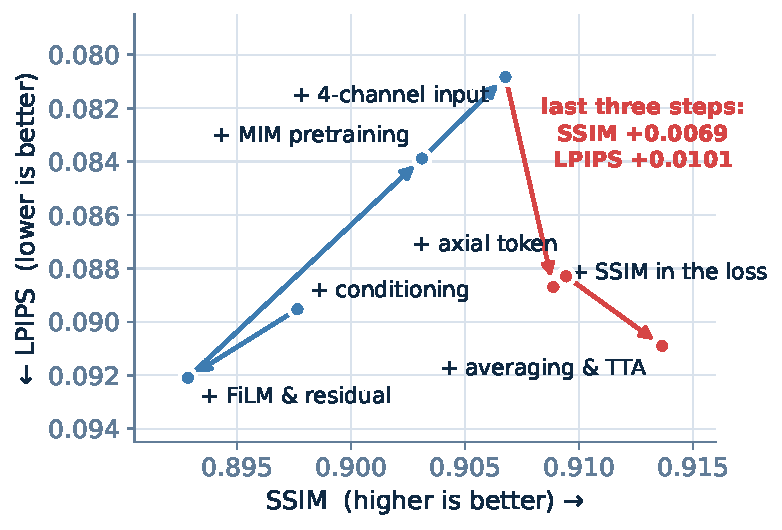
\includegraphics[width=\linewidth]{figures/showcase/trade_ladder_2.pdf}\\[-0.5mm]
  {\small a $\cdot$ validation: our submissions}
\end{minipage}\hfill
\begin{minipage}[t]{0.48\textwidth}\centering
  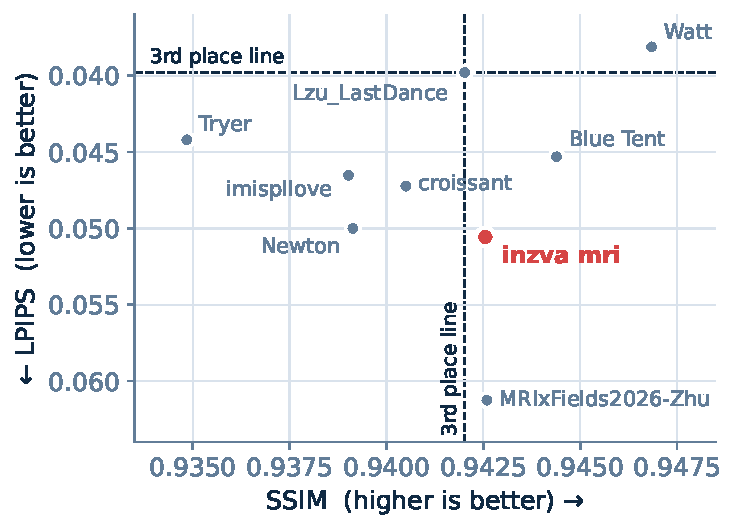
\includegraphics[width=\linewidth]{figures/showcase/trade_final.pdf}\\[-0.5mm]
  {\small b $\cdot$ test: the top 9}
\end{minipage}
\caption{SSIM against LPIPS, LPIPS axis inverted so up and right are better. Dashed lines in b:
SSIM and LPIPS of the 3rd-placed team.}
\label{fig:trade}
\end{figure}

\begin{itemize}
  \item SSIM was the main metric; the final place averages the ranks of all three metrics.
  \item We are 4th on SSIM, 0.00004 behind 3rd (MRIxFields2026-Zhu, 0.942594) and 0.00053 ahead
        of 5th (Lzu\_LastDance, 0.942018).
  \item LPIPS (14th) is the weak rank. On validation, the last three steps raised SSIM by 0.0069
        and worsened LPIPS by 0.0101 (Figure~\ref{fig:trade}.a): the SSIM loss term ($+0.0079$
        LPIPS) and averaging ($+0.0026$) both smooth.
\end{itemize}

% ======================================================================
\section{The model and the line that built it}\label{sec:model}

\begin{itemize}
  \item \textbf{Network}: 2D U-Net, 32 base channels, 4 levels; one axial slice in, one out.
  \item \textbf{Conditioning}: learned embeddings of the source and the target domain (15
        contrast $\times$ field domains) and a sinusoidal embedding of the slice's axial
        position, summed at the bottleneck and applied by zero-initialised FiLM in every decoder
        block; a zero-initialised residual head predicts a correction to the input.
  \item \textbf{Pretraining}: the whole network, by in-painting (50\% of 16\,px blocks zeroed,
        $L_1$ on the holes, the volume's own domain as condition), 30{,}000 steps on the 1{,}939
        retrospective volumes, which have no paired target.
  \item \textbf{Input}: four channels at the source field: the image being translated, then T1W,
        T2W and T2FLAIR.
  \item \textbf{Loss}: $L_1 + 0.5\,(1-\mathrm{SSIM}) + 0.05\,\mathrm{LPIPS}$, with the scorer's
        SSIM (7$\times$7 uniform window, validated against skimage to $3\cdot10^{-7}$).
  \item \textbf{Inference}: mean of the epoch 6, 7 and 8 weights; prediction averaged over the four
        in-plane flips; background zeroed where the source is below $10^{-3}$.
  \item Every added component is zero-initialised, so each run starts at its parent's exact
        function and any movement is the change, not the initialisation.
\end{itemize}

\begin{figure}[H]
\centering
\begin{subfigure}[t]{0.32\textwidth}\centering
  \unet{%
    \draw[->,draw=accent,line width=0.9pt,>={Stealth[length=1.6mm]}]
      (in) to[out=55,in=125] (out);
    \node[tag,align=center] at (8,8) {no network at all: $\hat{y}=x$};
  }
  \caption*{\panel{0 · copy the source}{0.836497}\\[0.5mm]
  \footnotesize Submitted deliberately. Source and target are the same registered subject,
  so the anatomy is free: this is the number every model has to beat.}
\end{subfigure}\hfill
\begin{subfigure}[t]{0.32\textwidth}\centering
  \unet{}
  \caption*{\panel{1 · vanilla U-Net}{0.869856}\\[0.5mm]
  \footnotesize Textbook U-Net, BatchNorm+ReLU, transposed-conv upsampling. It is never told
  which field pair it is being asked for. \textcolor{muted}{+0.0334}}
\end{subfigure}\hfill
\begin{subfigure}[t]{0.32\textwidth}\centering
  \unet{%
    \condtokens
    \node[tag,align=center,text=cond] at (8,6) {two domain\\embeddings};
  }
  \caption*{\panel{2 · + conditioning}{0.897646}\\[0.5mm]
  \footnotesize \textcolor{cond}{Source and target embeddings} over the 15
  modality$\times$field domains, broadcast-added at the bottleneck. \textcolor{cond}{+0.0278}}
\end{subfigure}

\vspace{2.5mm}

\begin{subfigure}[t]{0.32\textwidth}\centering
  \unet{%
    \condtokens
    \foreach \i/\w in {0/9,1/7,2/5,3/3.5}{\node[blk,hot,minimum width=\w mm] at (d\i) {};}
    \node[tag] at (19,6) {FiLM};
    \draw[->,draw=accent,line width=0.4pt,>={Stealth[length=1mm]}] (19,4.6) -- (17.5,1.8);
    \node[draw=accent,fill=accentfill,line width=0.6pt,rounded corners=0.4pt,
          font=\tiny,text=accent,inner sep=0.7pt] at (21,-6) {$x+f(x)$};
  }
  \caption*{\panel{3 · + FiLM \& residual}{0.892839}\\[0.5mm]
  \footnotesize Zero-init FiLM after both norms of every \emph{decoder} block; the head predicts a
  correction to the input instead of the image. Both are exact no-ops at step 0.}
\end{subfigure}\hfill
\begin{subfigure}[t]{0.32\textwidth}\centering
  \unet{%
    \condtokens
    \foreach \i/\w in {0/9,1/7,2/5,3/3.5}{
      \node[blk,hot,minimum width=\w mm] at (e\i) {};
      \node[blk,hot,minimum width=\w mm] at (d\i) {};}
    \node[blk,hot,minimum width=3mm] at (b) {};
    % input: the same image with half its blocks zeroed; output: the image itself
    \fill[white] (-9.5,-1.8) rectangle (-5.2,2);
    \foreach \r in {0,1,2}{\foreach \c in {0,1,2}{
      \fill[fill=baseline] ({-8.8+\c},{-1.5+\r}) rectangle ++(0.9,0.9);}}
    \foreach \r/\c in {0/1,1/0,1/2,2/1}{\fill[ink] ({-8.8+\c},{-1.5+\r}) rectangle ++(0.9,0.9);}
    \node[font=\tiny,text=muted,inner sep=0pt] at (-7.3,-2.6) {masked};
    \fill[white] (20.8,-1.8) rectangle (24,2);
    \foreach \r in {0,1,2}{\foreach \c in {0,1,2}{
      \fill[fill=baseline] ({21+\c},{-1.5+\r}) rectangle ++(0.9,0.9);}}
    \node[font=\tiny,text=muted,inner sep=0pt] at (22.5,-2.6) {full};
    \node[tag,align=center] at (8,7.5) {whole network pretrained by MIM\\on 1{,}939 unpaired volumes};
  }
  \caption*{\panel{4 · + MIM pretraining}{0.903110}\\[0.5mm]
  \footnotesize Identical network, every weight pretrained (not the encoder alone) by
  in-painting: 50\% of 16\,px blocks zeroed, $L_1$ on the holes, its own domain as condition, 30k
  steps on the \emph{retrospective} split, which has no paired target. Then the same weights are
  fine-tuned on the three paired subjects. \textcolor{accent}{+0.0103}}
\end{subfigure}\hfill
\begin{subfigure}[t]{0.32\textwidth}\centering
  \unet{%
    \condtokens
    \node[blk,hot,minimum width=9mm] at (e0) {};
    \foreach \k/\lab in {0/{$x$},1/{T1},2/{T2},3/{FL}}{
      \node[blk,hot,minimum width=2.4mm,minimum height=1.6mm] (ch\k) at (-6,{2.4-\k*2}) {};
      \node[font=\tiny,text=muted,inner sep=0.4pt,left=0.3mm of ch\k] {\lab};}
    \draw[->,draw=accent,line width=0.4pt,>={Stealth[length=1mm]}] (ch1) -- (e0);
    \node[tag,align=center] at (-2,8) {1\,$\to$\,4 input channels};
  }
  \caption*{\panel{5 · + multi-contrast}{\textcolor{accent}{0.906773}}\\[0.5mm]
  \footnotesize All three contrasts at the source field. Channel 0 duplicates the contrast being
  predicted, so the old single-channel first conv transfers exactly. \textcolor{accent}{+0.0037}}
\end{subfigure}
\caption{The line that worked, first half (to 2026-09-08). Each panel keeps everything to its
left and changes one thing. The two steps that paid, conditioning and pretraining on unpaired
data, are the two that gave the network \emph{more information}, not more capacity.}
\label{fig:lineA}
\end{figure}

\vspace{-1mm}

% ============================================================ the line, continued
\begin{figure}[H]
\centering
\begin{subfigure}[t]{0.32\textwidth}\centering
  \unet{%
    \condtokens
    \node[draw=accent,fill=accentfill,line width=0.6pt,rounded corners=0.4pt,
          font=\tiny,text=accent,inner sep=0.7pt] (loss) at (21,-6) {$+\mathcal{L}_{\mathrm{SSIM}}$};
    \draw[->,draw=accent,line width=0.5pt,>={Stealth[length=1mm]}] (out) -- (loss);
    \node[tag,align=center] at (19,6) {the ranked metric\\in the loss, weight 0.5};
  }
  \caption*{\panel{6 · + SSIM in the loss}{0.908873}\\[0.5mm]
  \footnotesize The scorer's own SSIM (7$\times$7 uniform window, validated to $3\cdot10^{-7}$)
  at weight 0.5 next to $L_1$ and LPIPS. Buys SSIM and nRMSE, spends LPIPS ($+0.0079$).
  \textcolor{accent}{+0.0021}}
\end{subfigure}\hfill
\begin{subfigure}[t]{0.32\textwidth}\centering
  \unet{%
    \condtokens
    \node[draw=accent,fill=accentfill,rounded corners=0.4pt,minimum height=2.2mm,
          line width=0.5pt,font=\tiny,text=accent,inner sep=0.6pt] (z) at (16,-21) {$+E_z$};
    \draw[->,draw=accent,line width=0.5pt,>={Stealth[length=1mm]}] (z) -- (c);
    \node[tag,align=center] at (19.5,-14) {axial position\\(sinusoidal,\\zero-init)};
  }
  \caption*{\panel{7 · + axial token}{0.909433}\\[0.5mm]
  \footnotesize A sinusoidal embedding of the slice's normalised $z$ joins the two domain
  embeddings, read by every decoder FiLM. Same seed and schedule as 6.
  \textcolor{muted}{+0.0006}}
\end{subfigure}\hfill
\begin{subfigure}[t]{0.32\textwidth}\centering
  \unet{%
    \condtokens
    \foreach \i/\w in {0/9,1/7,2/5,3/3.5}{
      \node[blk,hot,minimum width=\w mm] at (e\i) {};
      \node[blk,hot,minimum width=\w mm] at (d\i) {};}
    \node[blk,hot,minimum width=3mm] at (b) {};
    \node[tag,align=center] at (14,7.5) {$\bar w=\tfrac13(w_6\!+\!w_7\!+\!w_8)$};
    \foreach \k/\lab in {0/{$x$},1/{$x^{\leftrightarrow}$},2/{$x^{\updownarrow}$},3/{$x^{\leftrightarrow\updownarrow}$}}{
      \node[blk,hot,minimum width=2.4mm,minimum height=1.6mm] (v\k) at (-6,{2.4-\k*2}) {};
      \node[font=\tiny,text=accent,inner sep=0.4pt,left=0.3mm of v\k] {\lab};}
    \draw[->,draw=accent,line width=0.4pt,>={Stealth[length=1mm]}] (v1) -- (e0);
    \node[tag,align=center] at (-5.5,8) {4 flips in,\\mean out};
  }
  \caption*{\panel{8 · + avg \& TTA}{\textcolor{accent}{0.913652}}\\[0.5mm]
  \footnotesize No training. Weights are the mean of epochs 6--8 of run 7; the input is
  predicted under all four in-plane flips and the four outputs averaged.
  \textcolor{accent}{+0.0042}}
\end{subfigure}
\caption{The line that worked, second half (2026-09-08 to 09-11). Panel 8 is the shipped
test-phase model. The two halves of 8 had both been measured locally, declined as too small
($+0.0008$ and $+0.0009$), and revived only after the local harness was found to be scoring the
wrong plane (Section~\ref{sec:measure}): on the challenge they are worth more together than any single change since
conditioning.}
\label{fig:lineB}
\end{figure}

\begin{figure}[H]
\centering
\begin{subfigure}[t]{0.32\textwidth}\centering
  \unet{%
    \condtokens
    \node[blk,hot,minimum width=9mm] at (e0) {};
    \foreach \k/\lab in {0/{$z\!-\!2$},1/{$z$},2/{$z\!+\!2$}}{
      \node[blk,hot,minimum width=2.4mm,minimum height=1.6mm] (s\k) at (-6,{1.4-\k*2}) {};
      \node[font=\tiny,text=muted,inner sep=0.4pt,left=0.3mm of s\k] {\lab};}
    \draw[->,draw=accent,line width=0.4pt,>={Stealth[length=1mm]}] (s1) -- (e0);
    \node[tag,align=center] at (-2,8) {4\,$\to$\,12 channels:\\three axial slices};
  }
  \caption*{\panel{a · 2.5D input}{0.909353}\\[0.5mm]
  \footnotesize The 4-contrast block repeated at $z\pm2$ (1\,mm), new channels zero-init from
  panel 6's weights. Sibling of 7, not its parent: $+0.0005$ over 6, $-0.0001$ under 7.}
\end{subfigure}\hfill
\begin{subfigure}[t]{0.32\textwidth}\centering
  \unet{%
    \condtokens
    \node[blk,hot,minimum width=9mm] at (e0) {};
    \foreach \k in {0,1,2}{
      \node[blk,hot,minimum width=2.4mm,minimum height=1.6mm] (s\k) at (-6,{1.4-\k*2}) {};}
    \draw[->,draw=accent,line width=0.4pt,>={Stealth[length=1mm]}] (s1) -- (e0);
    \node[draw=accent,fill=accentfill,rounded corners=0.4pt,minimum height=2.2mm,
          line width=0.5pt,font=\tiny,text=accent,inner sep=0.6pt] (z) at (16,-21) {$+E_z$};
    \draw[->,draw=accent,line width=0.5pt,>={Stealth[length=1mm]}] (z) -- (c);
    \node[tag,align=center] at (0,8) {2.5D \emph{and} the axial token};
  }
  \caption*{\panel{b · 2.5D + axial token}{0.908354}\\[0.5mm]
  \footnotesize Both context signals at once, seeded from the 2.5D checkpoint. $-0.0010$ under
  its parent: the two do not add.}
\end{subfigure}\hfill
\begin{subfigure}[t]{0.32\textwidth}\centering
  \unet{%
    \condtokens
    \node[tag,align=center] at (8,7) {nothing in red:\\same run as 6, epoch 12 not 8};
  }
  \caption*{\panel{c · 12 epochs instead of 8}{0.908645}\\[0.5mm]
  \footnotesize Chosen by every local check we had (+0.0005 pooled over 180 transitions). Lost
  $0.0002$ on the challenge and on all three metrics: the local checks ran on the wrong plane.}
\end{subfigure}

\vspace{2.5mm}

\begin{subfigure}[t]{0.32\textwidth}\centering
  \unet{%
    \condtokens
    \foreach \i/\w in {0/9,1/7,2/5,3/3.5}{
      \node[blk,hot,minimum width=\w mm] at (e\i) {};
      \node[blk,hot,minimum width=\w mm] at (d\i) {};}
    \node[blk,hot,minimum width=3mm] at (b) {};
    \node[tag,align=center] at (8,7.5) {$\tfrac12\bar w_{6\text{--}8}+\tfrac12 w'_8$\\two runs, one seed};
  }
  \caption*{\panel{d · 50/50 model soup}{0.913203}\\[0.5mm]
  \footnotesize Panel 8's average blended with epoch 8 of its control run (6). The runs differ by
  one config line, so there was nothing to decorrelate; the single point diluted the average.
  $-0.0004$ under 8.}
\end{subfigure}\hfill
\begin{subfigure}[t]{0.32\textwidth}\centering
  \unet{%
    \condtokens
    \foreach \i/\w in {0/9,1/7,2/5,3/3.5}{
      \node[draw=accent,dashed,line width=0.5pt,minimum width=\w mm,minimum height=2.4mm,
            inner sep=0pt,rounded corners=0.4pt] at (d\i) {};}
    \node[tag] at (19,6) {no FiLM};
    \draw[->,draw=accent,line width=0.4pt,>={Stealth[length=1mm]}] (19,4.6) -- (17.5,1.8);
    \node[draw=accent,dashed,line width=0.6pt,rounded corners=0.4pt,
          font=\tiny,text=accent,inner sep=0.7pt] (r) at (21,-6) {$x+f(x)$};
    \draw[accent,line width=0.6pt] (r.south west) -- (r.north east);
  }
  \caption*{\panel{e · the chain without 3}{0.901476}\\[0.5mm]
  \footnotesize Pretrain (12k) $\to$ fine-tune with FiLM and the residual head removed, nothing
  else changed. 3 had scored $-0.0048$ in its one controlled comparison; against the FiLM line at
  the same 12k pretraining steps (0.901633): $-0.0002$.}
\end{subfigure}\hfill
\begin{subfigure}[t]{0.32\textwidth}\centering
  \unet{%
    \condtokens
    \foreach \i/\w in {0/9,1/7,2/5,3/3.5}{
      \node[blk,hot,minimum width=\w mm] at (e\i) {};
      \node[blk,hot,minimum width=\w mm] at (d\i) {};}
    \node[blk,hot,minimum width=3mm] at (b) {};
    \draw[->,draw=accent,line width=0.7pt,>={Stealth[length=1.4mm]}]
      (out) to[out=90,in=90,looseness=0.55] (in);
    \node[tag,align=center] at (8,8.3) {$v_\theta(x_t,t)$, 5 Heun steps};
  }
  \caption*{\panel{f · conditional flow matching}{0.886725}\\[0.5mm]
  \footnotesize The rank-1 team's recipe end to end: degradation-bridge pretraining, flow
  matching, GAN refinement; same inputs and conditioning as 5. Worse on all three metrics.}
\end{subfigure}
\caption{Branches off the line, 2026-09-09 to 09-11. Top row: the same weights family with
more context or more epochs, each within $\pm0.001$ of the spine. Bottom row: three different
bets, ordered by how far they fell. The 2.5D input is the only one of the six that beat what it
branched from, by $+0.0005$, the same amount the axial token bought on the spine; the
two did not add.}
\label{fig:branches}
\end{figure}

\begin{table}[H]
\centering
\small\setlength{\tabcolsep}{4pt}
\begin{tabular}{cllrrr}
\toprule
Panel & Submission & Architecture & SSIM $\uparrow$ & nRMSE $\downarrow$ & LPIPS $\downarrow$ \\
\midrule
\multicolumn{6}{l}{\itshape the line that worked} \\
\ref{fig:lineA}.0 & \texttt{task3\_input\_validation}      & identity control                & 0.836497 & 0.521604 & 0.157279 \\
\ref{fig:lineA}.1 & \texttt{unet-vanilla}                  & vanilla U-Net                   & 0.869856 & 0.402221 & 0.119849 \\
    & \texttt{unet-unconditioned}            & same, conditioning ablated      & 0.869784 & 0.404143 & 0.120421 \\
\ref{fig:lineA}.2 & \texttt{unet\_conditioned\_50ep}       & + domain embeddings             & 0.897646 & 0.241173 & 0.089527 \\
\ref{fig:lineA}.3 & \texttt{unet\_film\_residual\_ep8}     & + FiLM + residual head          & 0.892839 & 0.263835 & 0.092091 \\
    & \texttt{retro\_pretrain\_film}         & + MIM pretrain (12k, 883 vol)   & 0.901633 & 0.242206 & 0.085563 \\
\ref{fig:lineA}.4 & \texttt{unet\_cond\_retro30k\_pro20ep} & + MIM pretrain (30k, 1939 vol)  & 0.903110 & 0.245574 & 0.083882 \\
\ref{fig:lineA}.5 & \texttt{unet\_multi\_contrast\_e20}    & + 4-channel input               & 0.906773 & 0.243607 & \textbf{0.080831} \\
\ref{fig:lineB}.6 & \texttt{unet\_multicontrast\_ssim\_ep8}& + SSIM in the loss              & 0.908873 & 0.241785 & 0.088697 \\
\ref{fig:lineB}.7 & \texttt{mc\_ssim\_slice\_e8}           & + axial-position token          & 0.909433 & 0.240994 & 0.088294 \\
\ref{fig:lineB}.8 & \textbf{\texttt{mc\_ssim\_slice\_avg\_tta}} & \textbf{+ avg e6--e8 + 4-flip TTA} & \textbf{0.913652} & \textbf{0.237970} & 0.090899 \\
\midrule
\multicolumn{6}{l}{\itshape branches off the line, each scored against its parent} \\
\ref{fig:branches}.a & \texttt{mc\_25d\_e10}                  & 2.5D input ($z\pm2$), 12 ch     & 0.909353 & 0.243669 & 0.086309 \\
\ref{fig:branches}.b & \texttt{mc\_25d\_slice\_ep8}           & 2.5D + axial-position token     & 0.908354 & 0.244712 & 0.084906 \\
\ref{fig:branches}.c & \texttt{mc\_ssim\_long\_ep12}          & SSIM loss, epoch 12 not 8       & 0.908645 & 0.245014 & 0.089011 \\
\ref{fig:branches}.d & \texttt{soup\_5050\_tta}               & 50/50 soup of avg + control e8  & 0.913203 & 0.238661 & 0.091041 \\
\ref{fig:branches}.e & \texttt{plain\_e15}                    & the chain without FiLM/residual & 0.901476 & 0.238425 & 0.086357 \\
\midrule
\multicolumn{6}{l}{\itshape alternative backbones and formulations, dropped} \\
    & \texttt{swin\_cond\_10ep}              & Swin UNETR 3D, 10 ep            & 0.831536 & 0.300152 & 0.171283 \\
\ref{fig:dropped}.a & \texttt{swin\_cond\_50ep}              & Swin UNETR 3D, 50 ep            & 0.858214 & 0.279713 & 0.145240 \\
\ref{fig:dropped}.c & \texttt{tubelet\_encoder\_unetr\_...}  & LeJEPA tubelet + UNETR          & 0.859000 & 0.265807 & 0.143556 \\
\ref{fig:branches}.f & \texttt{cfm\_adv10\_tta}               & flow matching, 3 stages + TTA   & 0.886725 & 0.294564 & 0.111045 \\
\midrule
\multicolumn{6}{l}{\itshape teammates, same team} \\
    & \texttt{task3}                         & not logged                      & 0.905596 & 0.230754 & 0.085095 \\
    & \texttt{task3-str16}                   & not logged                      & 0.904645 & 0.232368 & 0.085955 \\
    & \texttt{task3-16t16}                   & 3D U-Net, 2 ep                  & 0.894233 & 0.243576 & 0.096655 \\
    & \texttt{StS-T-lj-un-v1}                & LeJEPA tubelet, 2 ep            & 0.889338 & 0.238274 & 0.088918 \\
    & \texttt{task\_3\_overfit\_fix\_try\_8b}& FPS-Former, 203 ep              & 0.879531 & 0.247053 & 0.149198 \\
\ref{fig:dropped}.b & \texttt{vit\_256\_150}                 & ViT / DINOv3                    & 0.878918 & 0.248285 & 0.149620 \\
    & \texttt{delitubet}                     & not logged                      & 0.876630 & 0.248372 & 0.138818 \\
    & \texttt{vit\_100}                      & ViT / DINOv3                    & 0.869782 & 0.263875 & 0.152566 \\
    & \texttt{epoch\_30\_fpsformer}          & FPS-Former, 30 ep               & 0.864881 & 0.283937 & 0.156116 \\
    & \texttt{val\_task3}                    & StarGAN v2 (challenge baseline) & 0.739694 & 0.343583 & 0.154472 \\
\bottomrule
\end{tabular}
\caption{Every accepted 180/180 Task 3 submission from the \texttt{inzva\_mri} team, grouped as
the figures are. Panel = figure.panel.}
\end{table}

\begin{itemize}
  \item \textbf{Information, not capacity.} Every step that paid gave the network more to see:
        which domain pair ($+0.0278$), 1{,}939 unpaired volumes ($+0.0103$), the other two
        contrasts ($+0.0037$), the scored metric in the loss ($+0.0021$).
  \item \textbf{Then averaging, with no training: $+0.0042$}, the largest step since
        conditioning.
  \item \textbf{Context signals saturate at one.} Neighbouring slices $+0.0005$, the axial token
        $+0.0006$, both together $-0.0010$ under the 2.5D parent.
\end{itemize}

% ======================================================================
\section{Everything tried, as a tree}\label{sec:tree}

\begin{figure}[H]
\centering
\resizebox{!}{0.84\textheight}{%
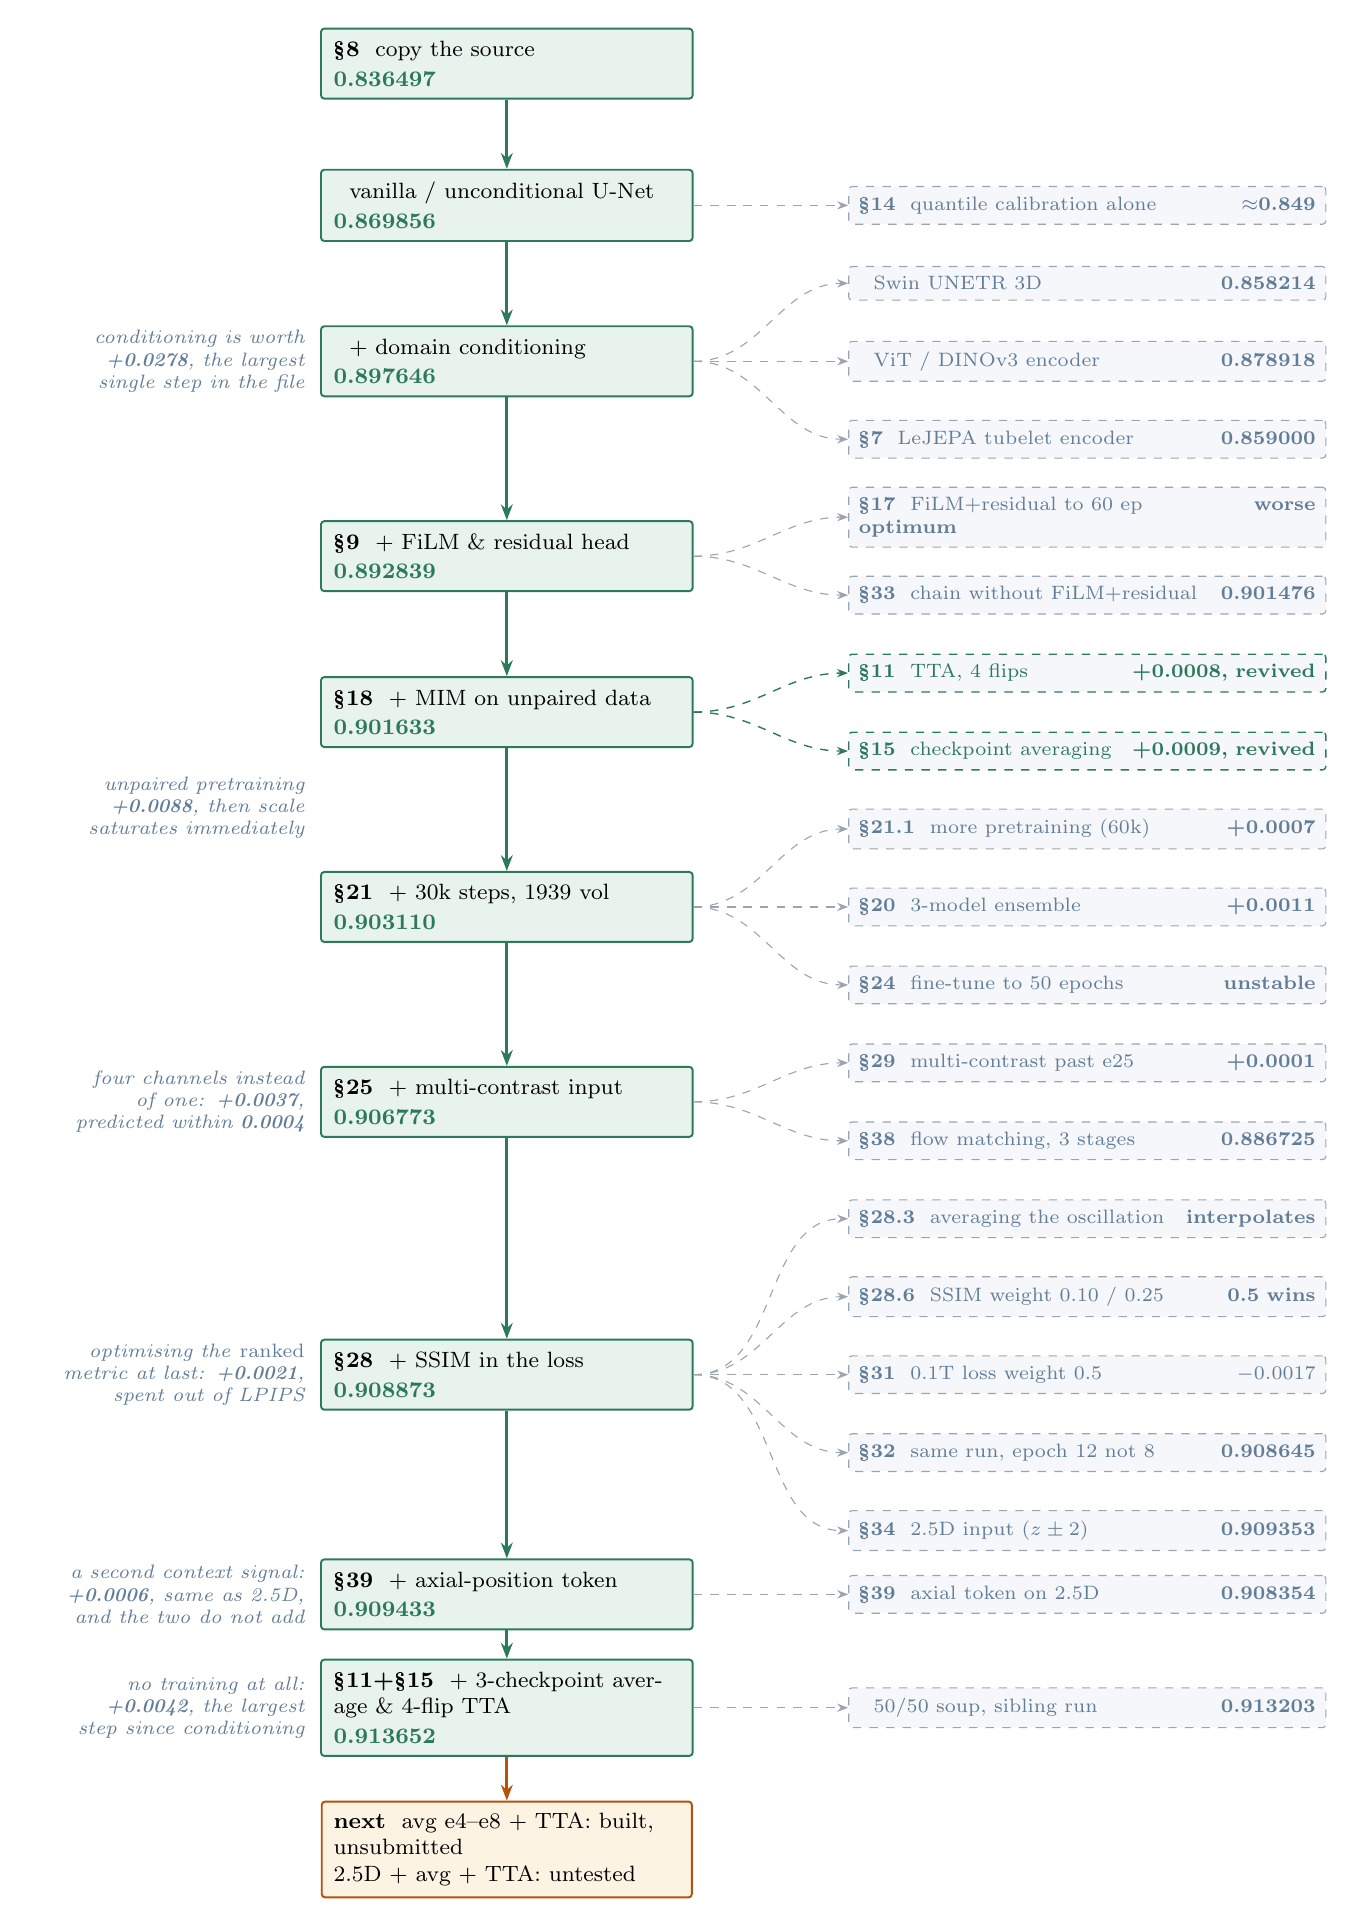
\begin{tikzpicture}[x=0.97cm,y=0.90cm]

% ------------------------------------------------------------------ the spine
\dtkept{n1}{0}      {\S8}   {copy the source}              {0.836497}
\dtkept{n2}{-2.0}   {}      {vanilla / unconditional U-Net} {0.869856}
\dtkept{n3}{-4.2}   {}      {+ domain conditioning}        {0.897646}
\dtkept{n4}{-6.95}  {\S9}   {+ FiLM \& residual head}      {0.892839}
\dtkept{n5}{-9.15}  {\S18}  {+ MIM on unpaired data}       {0.901633}
\dtkept{n6}{-11.9}  {\S21}  {+ 30k steps, 1939 vol}        {0.903110}
\dtkept{n7}{-14.65} {\S25}  {+ multi-contrast input}       {0.906773}
\dtkept{n8}{-18.5}  {\S28}  {+ SSIM in the loss}           {0.908873}
\dtkept{n9}{-21.6}  {\S39}  {+ axial-position token}       {0.909433}
\dtkept{n10}{-23.2} {\S11+\S15} {+ 3-checkpoint average \& 4-flip TTA} {0.913652}
\node[now] (n11) at (0,-25.2)
  {{\bfseries next}~~avg e4--e8 + TTA: built, unsubmitted\\
   2.5D + avg + TTA: untested};

\foreach \a/\b in {n1/n2, n2/n3, n3/n4, n4/n5, n5/n6, n6/n7, n7/n8, n8/n9, n9/n10}{\draw[spine] (\a) -- (\b);}
\draw[spine, draw=live] (n10) -- (n11);

% ------------------------------------------------------------------ dropped
\dtgone{d1}{-2.0}  {\S14} {quantile calibration alone}    {$\approx$0.849}
\dtgone{d2}{-3.1}  {}     {Swin UNETR 3D}                 {0.858214}
\dtgone{d3}{-4.2}  {}     {ViT / DINOv3 encoder}          {0.878918}
\dtgone{d4}{-5.3}  {\S7}  {LeJEPA tubelet encoder}        {0.859000}
\dtgone{d5}{-6.4}  {\S17} {FiLM+residual to 60 ep}        {worse optimum}
\dtgone{d6}{-7.5}  {\S33} {chain without FiLM+residual}   {0.901476}
\dtback{d7}{-8.6}  {\S11} {TTA, 4 flips}                  {+0.0008, revived}
\dtback{d8}{-9.7}  {\S15} {checkpoint averaging}          {+0.0009, revived}
\dtgone{d9}{-10.8} {\S21.1}{more pretraining (60k)}       {+0.0007}
\dtgone{d10}{-11.9}{\S20} {3-model ensemble}              {+0.0011}
\dtgone{d11}{-13.0}{\S24} {fine-tune to 50 epochs}        {unstable}
\dtgone{d12}{-14.1}{\S29} {multi-contrast past e25}       {+0.0001}
\dtgone{d13}{-15.2}{\S38} {flow matching, 3 stages}       {0.886725}
\dtgone{d14}{-16.3}{\S28.3}{averaging the oscillation}    {interpolates}
\dtgone{d15}{-17.4}{\S28.6}{SSIM weight 0.10 / 0.25}      {0.5 wins}
\dtgone{d16}{-18.5}{\S31} {0.1T loss weight 0.5}          {$-0.0017$}
\dtgone{d17}{-19.6}{\S32} {same run, epoch 12 not 8}      {0.908645}
\dtgone{d18}{-20.7}{\S34} {2.5D input ($z\pm2$)}          {0.909353}
\dtgone{d19}{-21.6}{\S39} {axial token on 2.5D}           {0.908354}
\dtgone{d20}{-23.2}{}     {50/50 soup, sibling run}       {0.913203}

\draw[stub] (n2.east) to[out=0,in=180] (d1.west);
\foreach \d in {d2,d3,d4}{\draw[stub] (n3.east) to[out=0,in=180] (\d.west);}
\foreach \d in {d5,d6}{\draw[stub] (n4.east) to[out=0,in=180] (\d.west);}
\foreach \d in {d7,d8}{\draw[ret] (n5.east) to[out=0,in=180] (\d.west);}
\foreach \d in {d9,d10,d11}{\draw[stub] (n6.east) to[out=0,in=180] (\d.west);}
\foreach \d in {d12,d13}{\draw[stub] (n7.east) to[out=0,in=180] (\d.west);}
\foreach \d in {d14,d15,d16,d17,d18}{\draw[stub] (n8.east) to[out=0,in=180] (\d.west);}
\draw[stub] (n9.east) to[out=0,in=180] (d19.west);
\draw[stub] (n10.east) to[out=0,in=180] (d20.west);

% ------------------------------------------------------------------ annotations
\dtnote{-4.2}  {conditioning is worth\\ \textbf{+0.0278}, the largest\\ single step in the file}
\dtnote{-10.5} {unpaired pretraining\\ \textbf{+0.0088}, then scale\\ saturates immediately}
\dtnote{-14.65}{four channels instead\\ of one: \textbf{+0.0037},\\ predicted within \textbf{0.0004}}
\dtnote{-18.5} {optimising the \emph{ranked}\\ metric at last: \textbf{+0.0021},\\ spent out of LPIPS}
\dtnote{-21.6} {a second context signal:\\ \textbf{+0.0006}, same as 2.5D,\\ and the two do not add}
\dtnote{-23.2} {no training at all:\\ \textbf{+0.0042}, the largest\\ step since conditioning}

\end{tikzpicture}
}
\caption{Task 3 to 2026-09-14. \textcolor{keep}{Green spine}: changes that shipped;
\textcolor{drop}{grey stubs}: tried and dropped; \textcolor{keep}{green dashed}: dropped on a
local number and later shipped; \textcolor{live}{orange}: built, not scored. Scores are
validation SSIM. The grey local deltas are pre-fix (Section~\ref{sec:measure}): read them as
signs at most.}
\label{fig:tree}
\end{figure}

\begin{itemize}
  \item \textbf{Two stubs came back.} TTA and checkpoint averaging read $+0.0008$ and $+0.0009$ on
        the pre-fix harness and were declined twice; submitted together they scored $+0.0042$.
  \item \textbf{The FiLM question.} FiLM and the residual head scored $-0.0048$ in their one
        controlled comparison, so the whole pretraining line was re-run without them [\S33]:
        0.901476, against 0.901633 for the FiLM line at the same 12k pretraining steps.
        Neither a cost nor a gain; closed.
  \item \textbf{Every stub is an architecture, a schedule or a second helping} of something on
        the spine. After this tree: \texttt{avg\_e4\_e8} + TTA is still unsubmitted, and 2.5D
        with averaging was never tried.
\end{itemize}

% ======================================================================
\section{Measurement}\label{sec:measure}

\textbf{The local harness scored the wrong plane until 2026-09-11} [\S41].
\begin{itemize}
  \item \texttt{eval\_holdout.py} walked axis 0 of the cached volume and fed every 2D model
        \emph{sagittal} $436\times364$ planes; training and the submission cut axial
        $364\times436$ ones. Both axes are 364 long and the network is fully convolutional, so
        nothing errored. The transpose existed only as an opt-in flag that the two tubelet
        configs set.
  \item A second drift: the eval scripts padded to $368\times448$ bottom-right, training and
        submission centre the pad, and InstanceNorm spreads the offset over the plane.
  \item Fixed by transposing unconditionally and centring the pad. Harness against the submission
        path on one slab: max $3.1\cdot10^{-4}$, mean $2.3\cdot10^{-6}$ (was mean
        $1.2\cdot10^{-2}$).
\end{itemize}

\begin{table}[H]
\centering\small
\begin{tabular}{lrr}
\toprule
Transition (\texttt{mc\_ssim\_slice} e8, subject 0006) & nRMSE, sagittal & nRMSE, axial \\
\midrule
T1W 3\,T$\to$7\,T        & 0.5422 & 0.1053 \\
T2FLAIR 1.5\,T$\to$7\,T  & 0.2545 & 0.1097 \\
T2W 7\,T$\to$0.1\,T      & 0.1669 & 0.0808 \\
\bottomrule
\end{tabular}
\caption{Same weights, only the input plane changed. nRMSE is a global voxel norm, so it reads
the error of the prediction itself, whichever plane a metric walks.}
\label{tab:plane}
\end{table}

\textbf{What it cost.}
\begin{itemize}
  \item TTA and checkpoint averaging were declined twice at $+0.0008$ / $+0.0009$; on the
        leaderboard they were worth $+0.0042$ together [\S11, \S15, \S40].
  \item Epoch 12 of the SSIM-loss run was preferred by every local check and lost 0.00023 on the
        leaderboard and on all three metrics [\S32].
  \item The local order of \texttt{mc\_ssim\_fine} and \texttt{mc\_ssim\_slice} was the reverse
        of the leaderboard's.
\end{itemize}

\textbf{What is void.} Pre-fix local results that this report does not quote as magnitudes:
seed spread (sd 0.0012) [\S16], spread across held-out subjects (sd 0.011) [\S14.1], the
``local cannot rank below 0.001'' ruler [\S32], 0.1\,T loss weighting ($-0.0017$) [\S31], the
3-model ensemble ($+0.0011$) [\S20], twice the pretraining ($+0.0007$) [\S21.1], the SSIM-weight
sweep [\S28.6], the long FiLM run [\S17], the local calibration offsets [\S8, \S22.1] and the
first error-by-field table [\S30]. Their signs may hold; their sizes are unknown.

\textbf{After the fix.}
\begin{table}[H]
\centering\small
\begin{tabular}{lrrr}
\toprule
Model & local slab SSIM & validation SSIM & offset \\
\midrule
\texttt{mc\_ssim\_fine} e8                       & 0.9536  & 0.908873 & 0.0447 \\
shipped, avg e6--e8 + TTA                         & 0.95069 & 0.913652 & 0.0370 \\
\bottomrule
\end{tabular}
\caption{The two models scored locally on the fixed harness (180 transitions, submission slab,
source-zeroed background).}
\label{tab:calib}
\end{table}
\begin{itemize}
  \item Locally the single checkpoint is ahead by 0.0029; on the leaderboard it is behind by
        0.0048. Local scoring is in-sample and rewards fit, so it still cannot rank models whose
        difference is generalisation.
  \item The leaderboard itself is stable: four teams' unmodified copies of the source scored
        0.836497 / 0.521604 to six decimals between 2026-06-16 and 08-28 [\S27].
\end{itemize}

% ======================================================================
\section{Where the error is}\label{sec:where}

\textbf{Two regimes in the data.} Radially averaged power spectra follow $P(f)\propto
f^{-\alpha}$; the slope gap to 7\,T is large only at 0.1\,T.

\begin{figure}[H]
\centering
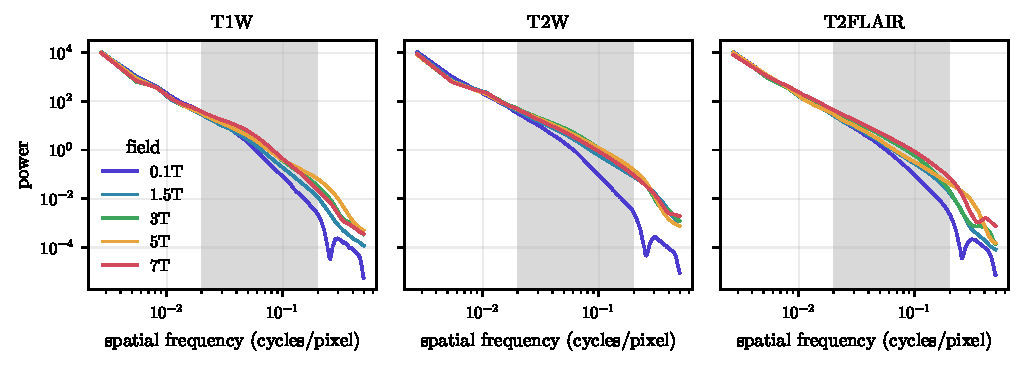
\includegraphics[width=0.86\textwidth]{spectral/fig_rapsd_by_field_retro.pdf}
\caption{Radially averaged power spectral density by field, per contrast, 30 retrospective
volumes per cell; slope fitted on 0.02--0.2 cycles/pixel (shaded).}
\label{fig:retro}
\end{figure}

\begin{table}[H]
\centering\small
\begin{tabular}{lccc}
\toprule
Source field & T1W & T2W & T2FLAIR \\
\midrule
0.1\,T & $\mathbf{+1.009}$ & $\mathbf{+1.502}$ & $\mathbf{+1.294}$ \\
1.5\,T & $+0.158$ & $+0.100$ & $+0.350$ \\
3\,T   & $-0.171$ & $-0.060$ & $+0.344$ \\
5\,T   & $-0.505$ & $-0.214$ & $+0.182$ \\
\bottomrule
\end{tabular}
\caption{$\alpha_{\text{source}} - \alpha_{7\,\mathrm{T}}$, retrospective split (Figure
\ref{fig:retro}). Positive: the source falls off faster, so detail has to be added.}
\label{tab:dalpha}
\end{table}

\begin{itemize}
  \item 0.1\,T sources lack most of 7\,T's fine detail; T1W and T2W sources at 3\,T and 5\,T are
        already finer than 7\,T, so translating among them mostly changes contrast.
  \item On the paired subjects, the best monotone pointwise intensity map between two fields
        explains 55--88\% of the variance and beats a straight line by at most 0.03 $R^2$; the
        rest is spatial, grey/white-matter structure in the difference maps [\S35].
\end{itemize}

\textbf{Error by field, shipped model, fixed harness.}
\begin{table}[H]
\centering\small
\begin{tabular}{lrrrr}
\toprule
& \multicolumn{2}{c}{as source} & \multicolumn{2}{c}{as target} \\
\cmidrule(lr){2-3}\cmidrule(lr){4-5}
Field & SSIM & share of error & SSIM & share of error \\
\midrule
\textbf{0.1\,T} & \textbf{0.9339} & \textbf{26.8\%} & \textbf{0.9424} & \textbf{23.4\%} \\
1.5\,T          & 0.9510 & 19.9\% & 0.9503 & 20.2\% \\
3\,T            & 0.9604 & 16.0\% & 0.9455 & 22.1\% \\
5\,T            & 0.9571 & 17.4\% & 0.9516 & 19.6\% \\
7\,T            & 0.9511 & 19.8\% & 0.9637 & 14.7\% \\
\bottomrule
\end{tabular}
\caption{Local slab SSIM and share of $\sum(1-\mathrm{SSIM})$, all 180 transitions (3 subjects
$\times$ 3 contrasts $\times$ 20 pairs), in-sample; mean 0.95069. Each share column sums to
100\%.}
\label{tab:byfield}
\end{table}

\begin{itemize}
  \item \textbf{0.1\,T is 40\% of the transitions and 50.2\% of the error}; transitions touching
        it score 0.9381 against 0.9590 for the rest.
  \item 7\,T is the easiest target (0.9637), 3\,T the easiest source (0.9604).
  \item \textbf{Direction makes no difference}: toward higher field 0.9506, toward lower 0.9508
        (90 transitions each). The pre-fix table [\S30] had read mapping up as easier; it does
        not hold.
  \item By contrast: T1W 0.9596, T2W 0.9516, T2FLAIR 0.9409.
\end{itemize}

\begin{figure}[H]
\centering
\begin{minipage}[t]{0.49\textwidth}\centering
  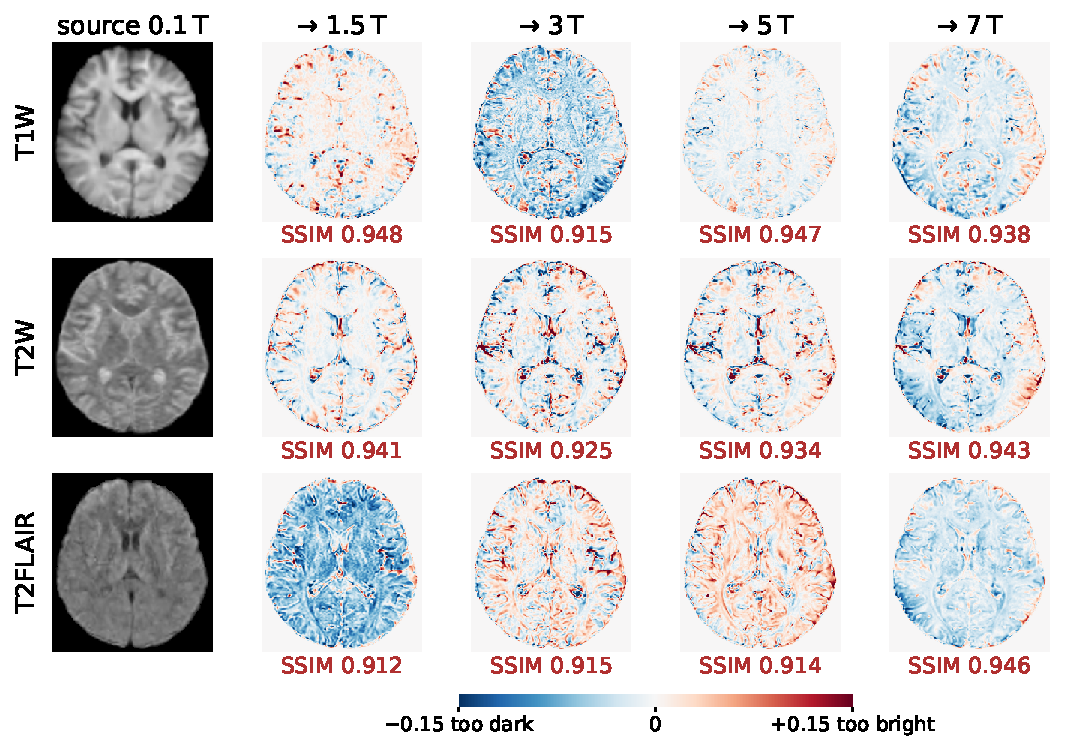
\includegraphics[width=\linewidth]{figures/showcase/grid_up_res.pdf}\\[-0.5mm]
  {\small a $\cdot$ from 0.1\,T to every higher field}
\end{minipage}\hfill
\begin{minipage}[t]{0.49\textwidth}\centering
  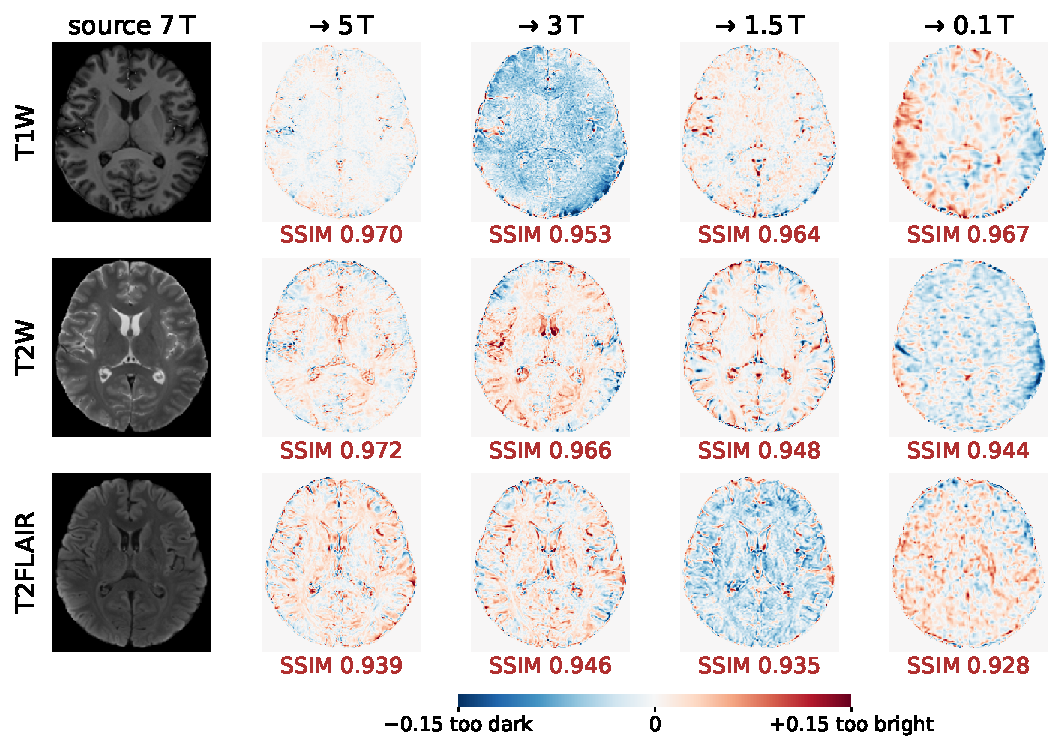
\includegraphics[width=\linewidth]{figures/showcase/grid_down_res.pdf}\\[-0.5mm]
  {\small b $\cdot$ from 7\,T to every lower field}
\end{minipage}
\caption{Prediction minus target, shipped weights with TTA, subject 0006 (in-sample), one axial
slice; slab SSIM under each. Blue: too dark; red: too bright.}
\label{fig:grids}
\end{figure}

% ======================================================================
\section{Error spectrum of the final model}\label{sec:spectrum}

\textbf{Setup} [\S44].
\begin{itemize}
  \item Shipped weights, 4-flip TTA, through the submission's own inference path; 3 subjects
        $\times$ 3 contrasts $\times$ 20 transitions on the submission slab; error
        $e = \hat y\cdot\mathbb{1}[x > 10^{-3}] - y$, the challenge's masking. 168 ranked
        transitions; in-sample, so read how the error splits, not its size.
  \item Radially averaged spectra of $e$, of $y$ and of the copy baseline's error $x - y$, per
        slice, zero-padded to square. Bands in cycles/pixel: low $<0.05$, mid 0.05--0.20,
        high $>0.20$.
  \item Space: $1-\mathrm{SSIM}$ maps and $e^2$; regions \emph{outer edge} (within 4\,px of the
        brain boundary), \emph{folds} (interior, top 20\% of $|\nabla y|$), \emph{flat} (the
        rest). Enrichment = error share / pixel share.
\end{itemize}

\begin{figure}[H]
\centering
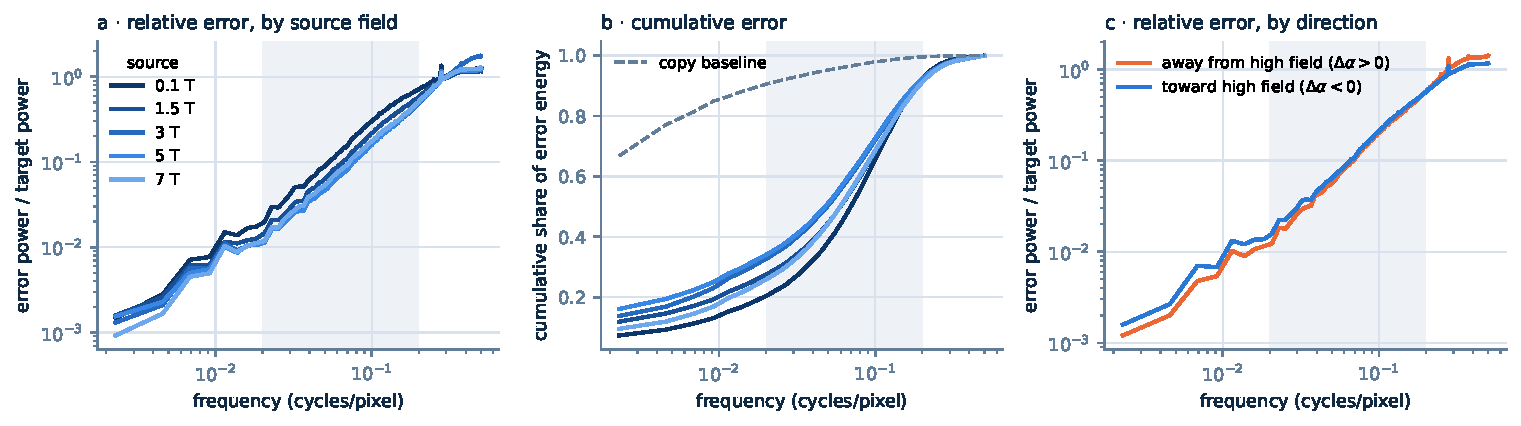
\includegraphics[width=\textwidth]{spectral/fig_error_rapsd_by_field.pdf}
\caption{Error spectrum. Shaded: the $\alpha$ fit band, 0.02--0.20 cycles/pixel.}
\label{fig:rapsd}
\end{figure}

\begin{table}[H]
\centering\small
\begin{tabular}{lllrrrrr}
\toprule
Panel & Quantity & Group & $<0.05$ & $0.05$--$0.1$ & $0.1$--$0.2$ & $0.2$--$0.3$ & $>0.3$ \\
\midrule
\ref{fig:rapsd}.a & $P_e / P_y$ & all            & 0.029 & 0.107 & 0.322 & 0.724 & 1.153 \\
\ref{fig:rapsd}.a & $P_e / P_y$ & source 0.1\,T  & 0.044 & 0.159 & 0.452 & 0.841 & 1.147 \\
\ref{fig:rapsd}.c & $P_e / P_y$ & $\da>0$ (away)   & 0.027 & 0.102 & 0.307 & 0.756 & 1.283 \\
\ref{fig:rapsd}.c & $P_e / P_y$ & $\da<0$ (toward) & 0.033 & 0.112 & 0.332 & 0.710 & 1.069 \\
\ref{fig:rapsd}.b & $P_e / P_{x-y}$ & all        & 0.10  & 0.26  & 0.42  & 0.54  & 0.61 \\
\bottomrule
\end{tabular}
\caption{Error power relative to the target (rows 1--4) and to the copy baseline's error
(row 5), per frequency band in cycles/pixel. The $<0.05$ column covers 0.02--0.05 only.}
\label{tab:bands}
\end{table}

\begin{itemize}
  \item \textbf{The low frequencies are solved.} The copy baseline's error is 96.7\% low band;
        the model's is 47.4\% low, 45.0\% mid, 7.6\% high (Figure~\ref{fig:rapsd}.b).
  \item \textbf{Relative error rises with frequency} at every source field: 3\% of the target's
        power at 0.02--0.05, 32\% at 0.1--0.2, above the target's own power past 0.3.
  \item \textbf{Direction does not separate the spectra}: away and toward overlap within 10\% in
        every band (Figure~\ref{fig:rapsd}.c). 0.1\,T as source sits 1.4--1.5$\times$ higher in
        the low and mid bands.
\end{itemize}

\begin{figure}[H]
\centering
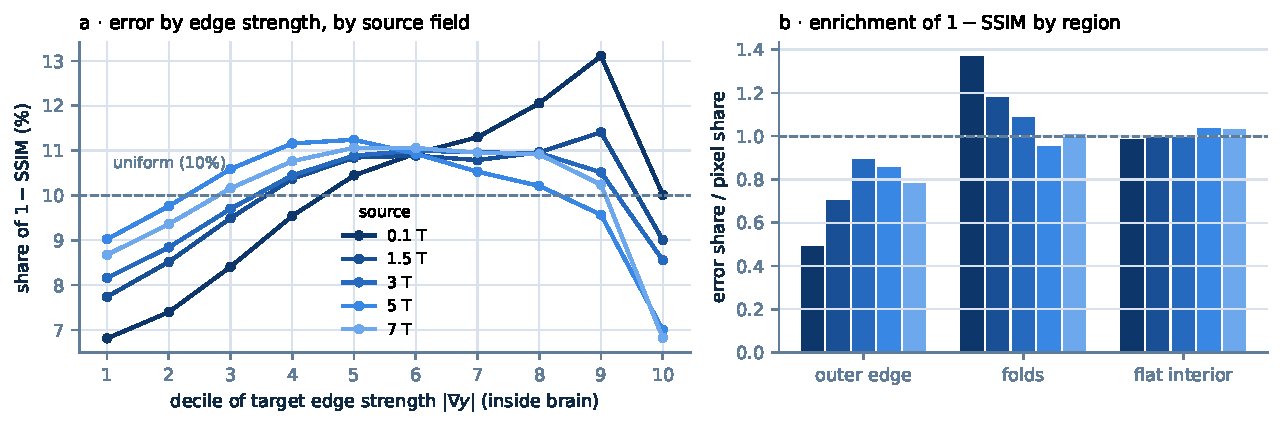
\includegraphics[width=0.92\textwidth]{spectral/fig_error_by_edge.pdf}
\caption{Spatial split of the ranked metric's deficit. Colours as in Figure~\ref{fig:rapsd}.a.}
\label{fig:edge}
\end{figure}

\begin{table}[H]
\centering\small
\begin{tabular}{llrrrrrr}
\toprule
Panel & Source & \multicolumn{3}{c}{$1-\mathrm{SSIM}$ enrichment} & top-2 deciles
      & $e^2$ folds & $\rho(|e|, |\nabla y|)$ \\
\cmidrule(lr){3-5}
 & & edge & folds & flat & of $1-\mathrm{SSIM}$ & enrichment & \\
\midrule
\ref{fig:edge}.b & all    & 0.71 & 1.14 & 1.00 & 19.7\% & 1.97 & 0.19 \\
\ref{fig:edge}.b & 0.1\,T & 0.49 & 1.36 & 0.98 & 23.1\% & 2.34 & 0.27 \\
\ref{fig:edge}.b & 1.5\,T & 0.69 & 1.17 & 0.99 & 20.4\% & 2.09 & 0.19 \\
\ref{fig:edge}.b & 3\,T   & 0.90 & 1.08 & 0.98 & 19.1\% & 1.73 & 0.17 \\
\ref{fig:edge}.b & 5\,T   & 0.85 & 0.94 & 1.03 & 16.6\% & 1.64 & 0.14 \\
\ref{fig:edge}.b & 7\,T   & 0.77 & 1.00 & 1.02 & 17.1\% & 1.79 & 0.20 \\
\bottomrule
\end{tabular}
\caption{Enrichment $=$ error share / pixel share (pixels: edge 10.3\%, folds 17.9\%, flat
71.7\%). Top-2 deciles: share of $1-\mathrm{SSIM}$ in the 20\% strongest-edge pixels.}
\label{tab:edge}
\end{table}

\begin{itemize}
  \item \textbf{Squared error follows the edges}: folds hold 35.3\% of $e^2$ on 17.9\% of the
        pixels, at every field.
  \item \textbf{The scored metric does not}: $1-\mathrm{SSIM}$ is spread like the pixels, 19.7\% in
        the top two edge deciles. SSIM divides by local variance, so an error on a high-contrast
        fold costs less than the same error on flat tissue.
  \item Only 0.1\,T and 1.5\,T as source put extra $1-\mathrm{SSIM}$ on folds (1.36, 1.17).
\end{itemize}

\begin{figure}[H]
\centering
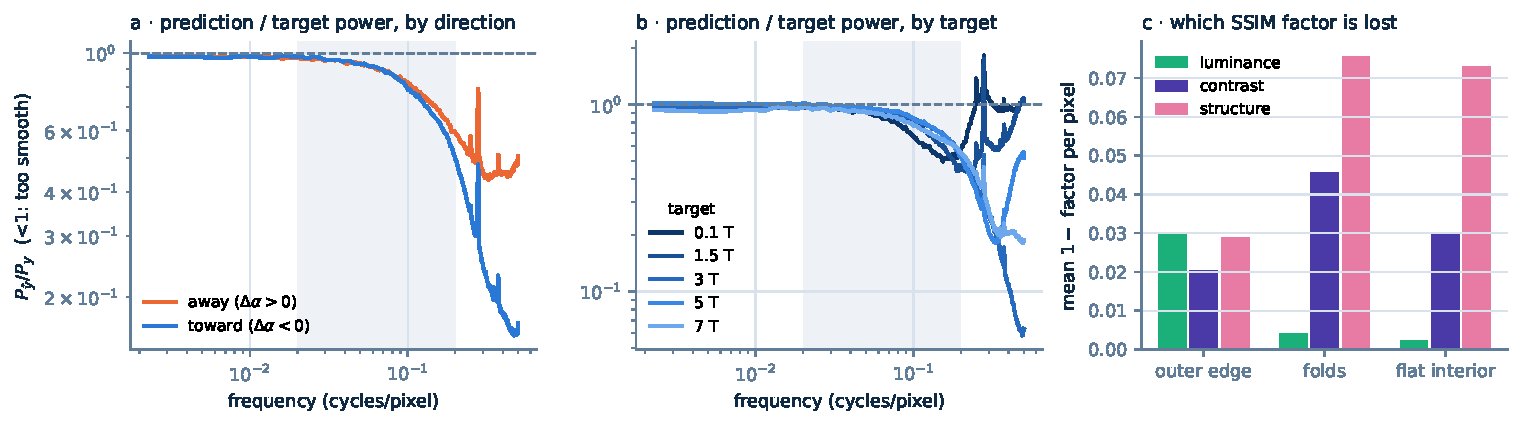
\includegraphics[width=\textwidth]{spectral/fig_error_smoothness.pdf}
\caption{Prediction power relative to the target, and the SSIM factor deficits by region.}
\label{fig:smooth}
\end{figure}

\begin{table}[H]
\centering\small
\begin{tabular}{llrrrrr}
\toprule
Panel & Group & $0.02$--$0.05$ & $0.05$--$0.1$ & $0.1$--$0.2$ & $0.2$--$0.3$ & $0.3$--$0.5$ \\
\midrule
\ref{fig:smooth}.a & all              & 0.958 & 0.893 & 0.715 & 0.447 & 0.299 \\
\ref{fig:smooth}.a & $\da>0$ (away)   & 0.955 & 0.896 & 0.743 & 0.546 & 0.453 \\
\ref{fig:smooth}.a & $\da<0$ (toward) & 0.961 & 0.891 & 0.697 & 0.401 & 0.200 \\
\ref{fig:smooth}.b & target 0.1\,T    & 0.947 & 0.843 & 0.592 & 0.866 & 0.974 \\
\ref{fig:smooth}.b & target 7\,T      & 0.940 & 0.866 & 0.693 & 0.461 & 0.218 \\
\bottomrule
\end{tabular}
\caption{$P_{\hat y}/P_y$ per band (cycles/pixel). Below 1: the prediction is smoother than
the target.}
\label{tab:smooth}
\end{table}

\begin{table}[H]
\centering\small
\begin{tabular}{llrrrrrr}
\toprule
Panel & Region & $1-l$ & $1-c$ & $1-s$ & $1-\mathrm{SSIM}$ & $\sigma^2_{\hat y}/\sigma^2_y$
      & smoother px \\
\midrule
\ref{fig:smooth}.c & outer edge    & 0.030 & 0.020 & 0.029 & 0.072 & 0.965 & 51\% \\
\ref{fig:smooth}.c & folds         & 0.004 & 0.046 & 0.076 & 0.115 & 0.791 & 77\% \\
\ref{fig:smooth}.c & flat interior & 0.002 & 0.030 & 0.073 & 0.101 & 0.856 & 69\% \\
\bottomrule
\end{tabular}
\caption{Mean per-pixel deficit of each SSIM factor ($l$ luminance, $c$ contrast, $s$
structure), all 168 transitions. Smoother px: share of windows with
$\sigma_{\hat y} < \sigma_y$.}
\label{tab:factors}
\end{table}

\begin{itemize}
  \item \textbf{Too smooth in every band, every group, both directions}: 0.715 of the target's
        power at 0.1--0.2 overall, 0.743 even away from high field. The one exception is target
        0.1\,T above 0.2 cycles/pixel, where the target is noise.
  \item \textbf{Structure is the largest SSIM loss} (0.073 in the flat interior, 0.076 on
        folds), \textbf{contrast the second}: 77\% of fold windows and 69\% of flat windows have
        $\sigma_{\hat y} < \sigma_y$. Over whole slices: luminance 0.0026, contrast 0.0149,
        structure 0.0322.
\end{itemize}

\subsection{Post-hoc sharpening: negative}\label{sec:e1}

\begin{itemize}
  \item For fixed covariance, $c\cdot s = (2\sigma_{\hat y y} + C_2)/(\sigma^2_{\hat y} +
        \sigma^2_y + C_2)$; scaling the prediction's local deviation by a gain $g$ leaves $s$
        unchanged and, for $C_2 \to 0$, peaks at $g = \sigma_y/\sigma_{\hat y}$, where $c = 1$.
        So SSIM could reward restoring the variance of detail the model already has.
  \item Tested without training: \emph{unsharp} masking ($g \in \{1.1, 1.2, 1.3, 1.5\}$,
        $\sigma \in \{1, 2\}$\,px) and \emph{window} gain on the 7$\times$7 deviation
        ($g \in \{1.05, 1.1, 1.2\}$, only where the local std exceeds
        $\tau \in \{0, 0.03, 0.06\}$): 17 settings.
\end{itemize}

\begin{table}[H]
\centering\small
\begin{tabular}{lrrrrr}
\toprule
Setting & $g$ & param & $\Delta$SSIM & $\Delta$nRMSE & improved \\
\midrule
window  & 1.05 & $\tau = 0.06$ & $-0.00005$ & $+0.00010$ & 24\% \\
window  & 1.05 & $\tau = 0.03$ & $-0.00006$ & $+0.00015$ & 26\% \\
unsharp & 1.1  & $\sigma = 1$  & $-0.00010$ & $+0.00015$ & 18\% \\
window  & 1.05 & $\tau = 0$    & $-0.00012$ & $+0.00021$ & 20\% \\
window  & 1.1  & $\tau = 0.06$ & $-0.00020$ & $+0.00031$ & 9\% \\
unsharp & 1.5  & $\sigma = 2$  & $-0.00550$ & $+0.00671$ & 0\% \\
\bottomrule
\end{tabular}
\caption{In-sample, 168 ranked transitions, against the shipped prediction (local SSIM 0.95113).
Best five of 17 settings plus the strongest; all 17 in \texttt{detail\_gain/grid.csv}.
Improved: share of transitions where the setting beats the shipped prediction.}
\label{tab:e1}
\end{table}

\begin{table}[H]
\centering\small
\begin{tabular}{lrrr}
\toprule
Rule & Held-out $\Delta$SSIM & $\Delta$nRMSE & improved \\
\midrule
one global setting                 & $0$         & $0$          & 0\% \\
one setting per target field       & $-0.00001$  & $+0.00002$   & 3\% \\
best setting per transition, oracle & $+0.00004$ & $+0.00001$   & 32\% \\
\bottomrule
\end{tabular}
\caption{Leave-one-subject-out: fit on two subjects, score on the third, all three rotations.
The global rule picks the identity in every fold; per target, only 7\,T picks a gain (window,
1.05) in two folds, and it loses on the held-out subject. The oracle is in-sample by
construction.}
\label{tab:e1loso}
\end{table}

\begin{itemize}
  \item \textbf{No setting raises SSIM}, globally, per target field or held out; the
        per-transition oracle is worth $+0.00004$.
  \item Why: 27--50\% of brain windows have $\sigma_y < 0.03 = \sqrt{C_2}$, where $C_2$ dominates;
        where $\sigma$ is large the per-window optimum varies too much for one gain. The contrast
        deficit is target variance the prediction cannot correlate with, not shrunken detail.
\end{itemize}

\subsection{$\Delta\alpha$-gated spectral-profile loss: negative}\label{sec:loss}

\begin{itemize}
  \item Report II's band-weighting idea, as a loss that acts only where the target is smoother
        than the source ($\da_{s\to t} = \alpha_t - \alpha_s > 0$), where the detail to remove
        is in the input:
\end{itemize}
\[
  \mathcal{L} = \mathcal{L}_{\text{shipped}}
  + \lambda\, \frac{1}{B}\sum_{b} \max(0, \da_b)\; \frac{1}{18}\sum_{r=1}^{18}
    \bigl|\log P_{\hat y_b}(r) - \log P_{y_b}(r)\bigr|,
  \qquad \lambda = 0.025,
\]
\begin{itemize}
  \item $P(r)$: \texttt{rfft2} power of the $368\times448$ training crop over ring $r$ (width 0.01
        cycles/pixel, 0.02--0.20), float32. $\lambda = 0.025$ makes the term 10\% of the loss at
        step 0.
  \item Same seed, start checkpoint and 8 epochs as the shipped run, which is the control; mean of
        e6--e8 and 4 flips; scored on the shipped model's local path (reproduced to $10^{-16}$).
\end{itemize}

\begin{table}[H]
\centering\small
\begin{tabular}{lrrrrrrrr}
\toprule
Epoch & 1 & 2 & 3 & 4 & 5 & 6 & 7 & 8 \\
\midrule
$1-\mathrm{SSIM}$, control  & 0.04411 & 0.04182 & 0.04081 & 0.03990 & 0.03919 & 0.03865 & 0.03808 & 0.03748 \\
$1-\mathrm{SSIM}$, spectral & 0.04487 & 0.04276 & 0.04171 & 0.04095 & 0.04025 & 0.03968 & 0.03915 & 0.03865 \\
gap                         & 0.00076 & 0.00094 & 0.00089 & 0.00106 & 0.00106 & 0.00103 & 0.00107 & 0.00117 \\
spectral term               & 0.0443  & 0.0363  & 0.0340  & 0.0324  & 0.0309  & 0.0300  & 0.0297  & 0.0288  \\
\bottomrule
\end{tabular}
\caption{Training-loss epoch means. The gated term falls from 0.164 at step 0 to 0.029, so the
network did learn it; the SSIM gap to the control opens in epoch 1 and never closes.}
\label{tab:spectrain}
\end{table}

\begin{table}[H]
\centering\small
\begin{tabular}{lrrrrrr}
\toprule
Group & $n$ & SSIM & $\Delta$SSIM & $\Delta$nRMSE & $\Delta$LPIPS & improved \\
\midrule
ranked              & 168 & 0.94995 & $-0.00118$ & $+0.00208$ & $+0.00034$ & 4 \\
gate on ($\da>0$)   & 81  & 0.95065 & $-0.00149$ & $+0.00216$ & $-0.00077$ & 2 \\
gate off ($\da<0$)  & 87  & 0.94929 & $-0.00089$ & $+0.00200$ & $+0.00138$ & 2 \\
target 0.1\,T       & 36  & 0.94008 & $-0.00232$ & $+0.00206$ & $+0.00044$ & 0 \\
target 7\,T         & 36  & 0.96287 & $-0.00080$ & $+0.00295$ & $-0.00044$ & 4 \\
\bottomrule
\end{tabular}
\caption{Local, paired per transition against the shipped model (ranked 0.95113). Improved:
transitions where SSIM rose; all four are 7\,T targets. Per modality: T1W $-0.00081$, T2W
$-0.00121$, T2FLAIR $-0.00153$.}
\label{tab:specscore}
\end{table}

\begin{figure}[H]
\centering
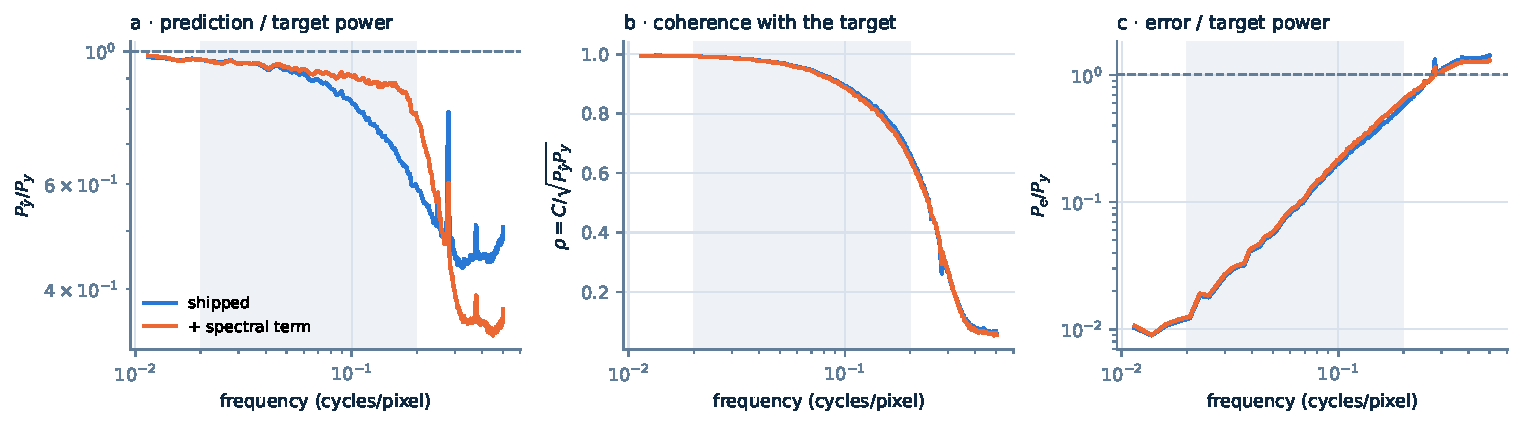
\includegraphics[width=\textwidth]{spectral/fig_spectral_loss.pdf}
\caption{Gate-on transitions (81 ranked), shipped against the spectral-loss model. Shaded: the
band the term acts on. $C = (P_{\hat y} + P_y - P_e)/2$ is the cross power, exact because
$e = \hat y - y$ is transformed on the same padded grid.}
\label{fig:specloss}
\end{figure}

\begin{table}[H]
\centering\small
\begin{tabular}{llrrr}
\toprule
Panel & Group, band (cycles/px) & $P_{\hat y}/P_y$ & coherence $\rho$ & $P_e/P_y$ \\
\midrule
\ref{fig:specloss} & gate on, 0.02--0.05 & 0.955 $\to$ 0.956 & 0.987 $\to$ 0.986 & 0.027 $\to$ 0.028 \\
\ref{fig:specloss} & gate on, 0.05--0.10 & 0.896 $\to$ 0.925 & 0.948 $\to$ 0.945 & 0.102 $\to$ 0.107 \\
\ref{fig:specloss} & gate on, 0.10--0.20 & 0.743 $\to$ 0.882 & 0.833 $\to$ 0.822 & 0.307 $\to$ 0.339 \\
\ref{fig:specloss} & gate on, 0.20--0.30 & 0.546 $\to$ 0.633 & 0.535 $\to$ 0.533 & 0.756 $\to$ 0.785 \\
                   & target 0.1\,T, 0.10--0.20 & 0.592 $\to$ 1.000 & 0.643 $\to$ 0.639 & 0.603 $\to$ 0.722 \\
                   & gate off, 0.10--0.20 & 0.697 $\to$ 0.670 & 0.818 $\to$ 0.815 & 0.332 $\to$ 0.336 \\
\bottomrule
\end{tabular}
\caption{Shipped $\to$ spectral-loss model, ring energies summed over the group's ranked
transitions (\texttt{error\_spectrum\_analysis.py} run on both). Full table in
\texttt{spectral\_loss/bands.csv}.}
\label{tab:specbands}
\end{table}

\begin{itemize}
  \item \textbf{The term did what it asks}: on gated transitions the 0.1--0.2 power rose from 0.743
        to 0.882 of the target's.
  \item \textbf{None of the added power is coherent with the target}: coherence 0.833 $\to$ 0.822,
        so the error rose with the power (0.307 $\to$ 0.339).
  \item \textbf{SSIM falls most where the term acts}: gate on $-0.00149$, target 0.1\,T $-0.00232$;
        164 of 168 transitions lower. Ungated transitions also lost $-0.00089$.
  \item LPIPS improves only where the term acts ($-0.00077$, gate on).
  \item \textbf{Closed}: with the sharpening result, the missing power is not coherent with
        anything in the input the network can reach. More SSIM needs information, not another
        loss shape.
\end{itemize}

% ======================================================================
\section{Other routes}\label{sec:other}

\begin{figure}[H]
\centering
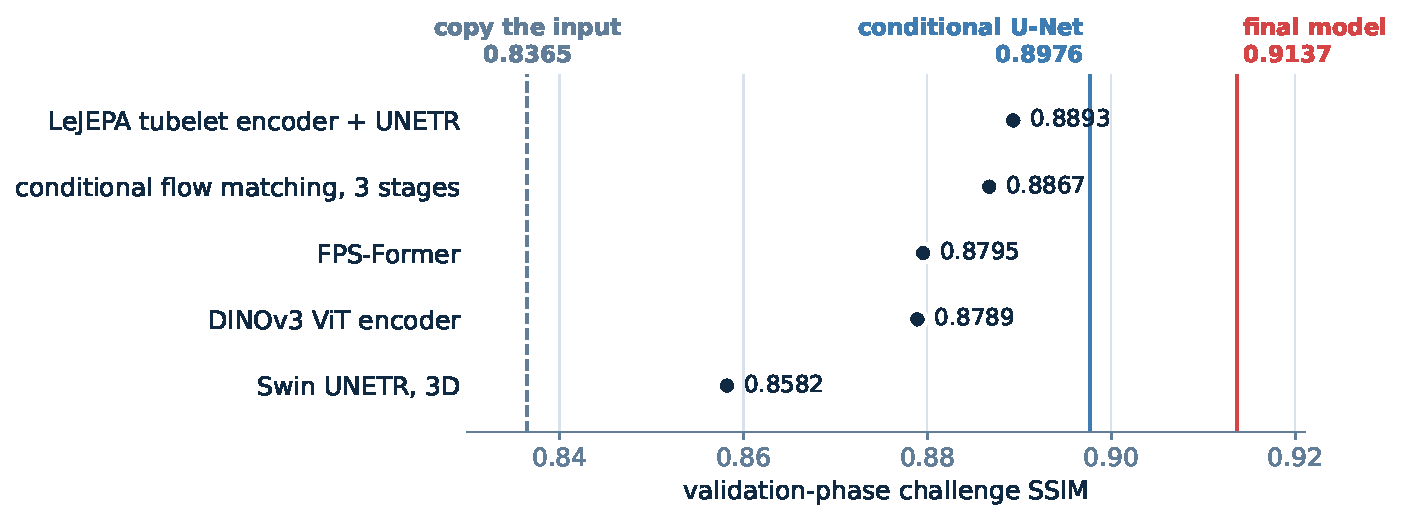
\includegraphics[width=0.82\textwidth]{figures/showcase/other_backbones.pdf}
\caption{The five other backbones and formulations, validation SSIM, against the U-Net line.}
\label{fig:backbones}
\end{figure}

\begin{figure}[H]
\centering
\begin{subfigure}[t]{0.32\textwidth}\centering
  \unet{%
    \foreach \i/\w in {0/9,1/7,2/5,3/3.5}{\node[blk,hot,minimum width=\w mm] at (e\i) {};}
    \node[blk,hot,minimum width=3mm] at (b) {};
    \node[tag,align=center] at (6,7) {Swin-T encoder,\\volumetric};
    \node[tag,text=cond] at (20,-20) {re-injected};
    \draw[->,draw=cond,line width=0.4pt,>={Stealth[length=1mm]}] (20,-18.6) -- (17,-13);
  }
  \caption*{\panel{a · Swin UNETR 3D}{0.858214}\\[0.5mm]
  \footnotesize Shifted-window transformer encoder on volumes. Conditioning had to be re-injected
  in the decoder; a bottleneck add does not survive the norms.}
\end{subfigure}\hfill
\begin{subfigure}[t]{0.32\textwidth}\centering
  \unet{%
    \foreach \i/\w in {0/9,1/7,2/5,3/3.5}{\node[blk,hot,minimum width=\w mm] at (e\i) {};}
    \node[blk,hot,minimum width=3mm] at (b) {};
    \node[tag,align=center] at (6,7) {frozen DINOv3 ViT,\\natural images};
  }
  \caption*{\panel{b · ViT / DINOv3}{0.878918}\\[0.5mm]
  \footnotesize Pretrained natural-image features reassembled by a conv decoder. Teammate's run.}
\end{subfigure}\hfill
\begin{subfigure}[t]{0.32\textwidth}\centering
  \unet{%
    \foreach \i/\w in {0/9,1/7,2/5,3/3.5}{\node[blk,hot,minimum width=\w mm] at (e\i) {};}
    \node[blk,hot,minimum width=3mm] at (b) {};
    \node[tag,align=center] at (6,7) {LeJEPA tubelet encoder,\\axial slabs};
  }
  \caption*{\panel{c · Tubelet + UNETR}{0.859000}\\[0.5mm]
  \footnotesize Self-supervised video-style encoder on axial slabs, conditioned UNETR decoder.}
\end{subfigure}
\caption{Backbones tried and dropped. In each case the \textcolor{accent}{encoder} is replaced
and the decoder kept. All three are stronger feature extractors than a 32-channel U-Net and all
three scored \emph{worse}: with three paired training subjects, encoder capacity is not the
binding constraint.}
\label{fig:dropped}
\end{figure}

\begin{itemize}
  \item \textbf{LeJEPA tubelet encoder} [\S3, \S7]. The CLS path trained well (effective rank
        $+66$ over random initialisation, retrieval top-1 0.883--0.983). The dense tokens the
        decoder reads lost 70 points of effective rank against random initialisation, and a
        matched location is only 0.0177 more similar than a wrong one. The submission also
        carried two artifacts: a 16\,px patch grid (error power 709$\times$ the median at
        16.15\,px) and slab seams (z-gradient 2.17$\times$ at every 16th slice).
  \item \textbf{FPS-Former}, 203 epochs: 0.879531 / 0.247053 / 0.149198. 30 epochs had scored
        0.864881.
  \item \textbf{Conditional flow matching} [\S38, \S40], the recipe of the then rank-1
        validation team (arXiv:2609.00960), reproduced end to end: degradation-bridge
        pretraining (25k steps, 232{,}320 retrospective slices), flow matching (4{,}120 steps),
        adversarial refinement (11{,}000 steps), 5 Heun steps and 4 flips. 0.886725 / 0.294564 /
        0.111045, worse than the U-Net line on all three metrics. The paper's own best is 0.909.
  \item \textbf{Synthetic pairs from degraded 7\,T}: built in Report II, never trained on (Table
        \ref{tab:plans}).
\end{itemize}

\begin{table}[H]
\centering\small
\begin{tabular}{llrr}
\toprule
Change & parent & SSIM & $\Delta$ \\
\midrule
2.5D input, slices $z\pm2$            & SSIM-loss run, e8      & 0.909353 & $+0.00048$ \\
axial token on the 2.5D model          & 2.5D, e10              & 0.908354 & $-0.00100$ \\
epoch 12 instead of 8                  & SSIM-loss run, e8      & 0.908645 & $-0.00023$ \\
50/50 soup with a sibling run          & shipped                & 0.913203 & $-0.00045$ \\
no FiLM, no residual head (12k pretrain) & FiLM line, 12k pretrain & 0.901476 & $-0.00016$ \\
spectral-profile loss (local, fixed harness) & shipped        & 0.94995  & $-0.00118$ \\
\bottomrule
\end{tabular}
\caption{Changes to the U-Net line with a score against their parent. Validation SSIM except the
last row, which is local ranked-168 SSIM.}
\label{tab:changes}
\end{table}

% ======================================================================
\section{Test phase, data integrity and the workshop}\label{sec:test}

\begin{table}[H]
\centering\small
\begin{tabular}{lll}
\toprule
& validation phase & test phase \\
\midrule
volume shape & $364\times436\times30$, the \texttt{Z\_CLIP\_RANGE} slab & $364\times436\times364$,
  full volume \\
file list & our own subject table & \texttt{/input/manifest.json} only; case ids hidden \\
count & 180 & 120 (20 pairs $\times$ 2 cases $\times$ 3 contrasts) \\
delivery & ZIP to Synapse & Docker image, \texttt{docker.synapse.org/syn76236366/task3} \\
\bottomrule
\end{tabular}
\caption{What changed for the test phase [\S36].}
\label{tab:phases}
\end{table}

\begin{itemize}
  \item \textbf{Image v1} (2026-09-10) shipped \texttt{mc\_ssim\_fine} e8 (0.908873). \textbf{Image
        v2} (2026-09-11) ships the averaged e6--e8 weights with slice conditioning and 4-flip TTA,
        the 0.913652 model: 0 difference at module level, $1.8\cdot10^{-4}$ at the entrypoint
        [\S42].
  \item \textbf{Data Integrity Policy} [\S43]. The organisers asked for the training logs behind
        the submission. The original machine was gone, so the chain was re-executed on Colab from
        the same configs under the organisers' runtime monitor (preprocess, pretrain, widen,
        fine-tune, average, export, predict) and packaged as
        \texttt{audit/inzva\_mri-audit-materials.zip}.
  \item \textbf{Workshop.} 22 papers are on the challenge page; our team has none among them. The
        top teams' methods:
\end{itemize}

\begin{table}[H]
\centering\small
\begin{tabular}{@{}rlp{10.4cm}@{}}
\toprule
place & team & method (workshop paper) \\
\midrule
1 & Watt (MSRA) & source-conditioned translation with shared-cycle refinement \\
2 & Blue Tent (Warwick) & latent bridge matching: Stable Diffusion 2.1 VAE + Marigold U-Net,
  one step, LPIPS weight 0.2 \\
3 & Lzu\_LastDance (Lanzhou) & FieldMorphUNet, structure-scale decoupling \\
4 & croissant (NEUROPHET) & paired--synthetic--paired latent diffusion \\
5 & Newton (Leiden UMC) & conditional flow matching + adversarial refinement \\
6 & inzva mri (ITU, inzva) & MIM pretraining + conditioning (this report) \\
8 & MRIxFields2026-Zhu (UW) & frozen DINOv3 + DPT decoder; FiLM output-stack cascade \\
\bottomrule
\end{tabular}
\caption{Methods of the top teams with a workshop paper. Blue Tent's and Newton's are on arXiv
(2609.20341, 2609.00960).}
\label{tab:teams}
\end{table}

% ======================================================================
\section{Deliverables}\label{sec:deliver}

\begin{itemize}
  \item \textbf{MICCAI talk} (\texttt{slides\_miccai}): 10 slides and a backup, 5 minutes,
        presented 1 October.
  \item \textbf{Showcase deck} (\texttt{showcase\_presentation\_v0}): about 15 minutes, 29 slides,
        a closing slide and 4 backups; problem and metrics, analyses, method and qualitative
        grids, error spectrum, other methods, results, fastMRI as future work. Workshop photo,
        preprint page and presenter initials still to add.
  \item \textbf{Preprint draft} (\texttt{reports/preprint/}, Springer LNCS): title, abstract and
        introduction written; the other sections planned.
  \item \textbf{Scripts}: \texttt{error\_spectrum\_analysis.py}, \texttt{detail\_gain\_sweep.py},
        \texttt{spectral\_loss\_eval.py}, \texttt{make\_showcase\_qualitative.py},
        \texttt{make\_showcase\_figures.py}, \texttt{make\_showcase\_explainers.py}.
\end{itemize}

% ======================================================================
\section{Open items}\label{sec:open}

\begin{itemize}
  \item Calibrate the fixed harness against the leaderboard: two points so far, ranked in opposite
        orders (Table~\ref{tab:calib}).
  \item Re-measure on the fixed harness the void results that decisions rested on: seed spread,
        held-out-subject spread, and 0.1\,T loss weighting, which closed the synthetic-pair route.
  \item Built, not submitted: \texttt{avg\_e4\_e8} + TTA, and the spectral-loss model. 2.5D with
        averaging and TTA never tried.
  \item The showcase deck's ``Error by field strength'' and ``Measurement limits'' slides still
        quote pre-fix local numbers; Tables~\ref{tab:byfield} and~\ref{tab:calib} have the
        current ones.
  \item Preprint: sections 2 to 8.
  \item Horizon B: the dense/CLS gap of the LeJEPA encoder [\S3] and a port to fastMRI [\S2].
\end{itemize}

\end{document}
